\chapter{Thực nghiệm và thảo luận}
\label{ch:thuc-nghiem}

Chương này trình bày toàn bộ kết quả thực nghiệm và các phân tích chuyên sâu nhằm trả lời 5 câu hỏi nghiên cứu (RQ1--RQ5) đã đặt ra. Các thực nghiệm được tổ chức theo mạch lập luận: (1) Đánh giá đóng góp của các nhóm đặc trưng ($F_1 \to F_4$); (2) Tinh chỉnh siêu tham số và khảo sát mô hình kết hợp; (3) Khảo sát sự suy giảm hiệu năng theo độ chi tiết nhãn ($T_2 \to T_5$); (4) Phân tích nguyên nhân suy thoái thông qua tương quan sinh hóa và chồng lấn hình học PCA; (5) Thử nghiệm mở rộng dữ liệu đa chu kỳ NHANES; (6) Khảo sát toàn diện 8 họ mô hình ($E_0 \to E_7$) trên không gian 3 nhóm ($T_3$); (7) Phân tích sự đánh đổi an toàn lâm sàng theo ma trận chi phí; (8) Kiểm định tính bền vững ngoại suy theo dòng thời gian; và (9) Thảo luận tổng hợp các phát hiện khoa học.

\section{Thiết lập thực nghiệm và kiểm soát tính khả lập}
\label{sec:moi-truong-thuc-nghiem}

Toàn bộ quá trình huấn luyện và kiểm định mô hình được thực hiện trong môi trường chuẩn tắc:
\begin{itemize}
    \item \textbf{Phần cứng:} Máy trạm Apple Silicon (ARM64, kiến trúc vi xử lý M-series), bộ nhớ 16 GB RAM, ổ cứng SSD tốc độ cao.
    \item \textbf{Hệ điều hành và môi trường phần mềm:} macOS Darwin Kernel 24.6.0; Python phiên bản 3.13 chạy trong môi trường ảo hóa độc lập (\texttt{.venv}).
    \item \textbf{Thư viện tính toán khoa học:} \texttt{scikit-learn} 1.9.1 (các thuật toán học máy, tiền xử lý và kiểm định chéo); \texttt{xgboost} 3.4.1 (tăng cường độ dốc cực đại); \texttt{scipy} 1.18.1 (tối ưu hóa phi tuyến L-BFGS-B cho mô hình OLR); \texttt{numpy} 2.5.3 và \texttt{pandas} 3.0.6 (xử lý ma trận và bảng dữ liệu); \texttt{matplotlib} 3.11.2 (trực quan hóa dữ liệu và xuất biểu đồ 300 DPI).
    \item \textbf{Kiểm soát tính ngẫu nhiên:} Hạt giống \texttt{random\_state = 42} được cố định nghiêm ngặt trên tất cả các phép chia fold, khởi tạo mô hình và lấy mẫu bootstrap nhằm triệt tiêu phương sai ngẫu nhiên giữa các lần chạy.
\end{itemize}

\section{Đánh giá đóng góp của các nhóm đặc trưng (Feature Ablation)}
\label{sec:feature-ablation}

\subsection{Thiết lập thực nghiệm}
Thực nghiệm Feature Ablation nhằm trả lời câu hỏi nghiên cứu \textbf{RQ1}: Khảo sát sự đóng góp thực tế của bốn nhóm đặc trưng lũy tiến ($F_1 \to F_4$) đối với bài toán 5 lớp chuẩn $T_5$ ($C_0 \to C_4$). Thực nghiệm được thực hiện thông qua Stratified 5-Fold Cross-Validation trên tập phát triển Legacy ($N = 4.045$). Bốn thuật toán học máy cơ sở được đánh giá song song gồm: Hồi quy Logistic (LR), Cây quyết định (DT), Rừng ngẫu nhiên (RF) và eXtreme Gradient Boosting (XGBoost).

\subsection{Kết quả thực nghiệm}
Kết quả out-of-fold chi tiết được tổng hợp trong Bảng \ref{tab:ablation-results}. Hình \ref{fig:ablation-comparison} trực quan hóa xu hướng biến thiên của Macro-F1 trên các không gian đặc trưng.

\begin{table}{Kết quả thực nghiệm Feature Ablation trên tập Legacy Development ($N = 4.045$, 5 lớp $T_5$)}
\centering
\footnotesize
\setlength{\tabcolsep}{3pt}
\label{tab:ablation-results}
\begin{tabularx}{\textwidth}{l c l >{\centering\arraybackslash}X >{\centering\arraybackslash}X >{\centering\arraybackslash}X}
\toprule
\textbf{Nhóm} & \textbf{$d$} & \textbf{Mô hình ML} & \textbf{Macro-F1 (Mean $\pm$ SD)} & \textbf{Balanced Acc (Mean $\pm$ SD)} & \textbf{Weighted-F1 (Mean $\pm$ SD)} \\
\midrule
\multirow{4}{*}{\textbf{$F_1$}} & \multirow{4}{*}{10} 
  & Logistic Regression & 0.1900 $\pm$ 0.0164 & 0.2420 $\pm$ 0.0299 & 0.4926 $\pm$ 0.0209 \\
& & Decision Tree        & 0.2081 $\pm$ 0.0121 & 0.2090 $\pm$ 0.0133 & 0.5926 $\pm$ 0.0081 \\
& & Random Forest       & 0.2052 $\pm$ 0.0072 & 0.2090 $\pm$ 0.0065 & 0.6314 $\pm$ 0.0107 \\
& & XGBoost             & 0.2173 $\pm$ 0.0147 & 0.2295 $\pm$ 0.0220 & 0.5577 $\pm$ 0.0072 \\
\midrule
\multirow{4}{*}{\textbf{$F_2$}} & \multirow{4}{*}{19} 
  & Logistic Regression & 0.2338 $\pm$ 0.0041 & 0.2942 $\pm$ 0.0299 & 0.5648 $\pm$ 0.0092 \\
& & Decision Tree        & 0.2319 $\pm$ 0.0154 & 0.2357 $\pm$ 0.0185 & 0.6144 $\pm$ 0.0093 \\
& & Random Forest       & 0.2350 $\pm$ 0.0180 & 0.2353 $\pm$ 0.0155 & 0.6557 $\pm$ 0.0097 \\
& & XGBoost             & 0.2447 $\pm$ 0.0143 & 0.2594 $\pm$ 0.0187 & 0.6002 $\pm$ 0.0123 \\
\midrule
\multirow{4}{*}{\textbf{$F_3$}} & \multirow{4}{*}{29} 
  & Logistic Regression & 0.2390 $\pm$ 0.0084 & 0.3194 $\pm$ 0.0284 & 0.5637 $\pm$ 0.0071 \\
& & Decision Tree        & 0.2388 $\pm$ 0.0127 & 0.2408 $\pm$ 0.0148 & 0.6195 $\pm$ 0.0100 \\
& & Random Forest       & 0.2299 $\pm$ 0.0045 & 0.2314 $\pm$ 0.0047 & 0.6671 $\pm$ 0.0085 \\
& & XGBoost             & 0.2588 $\pm$ 0.0402 & 0.2713 $\pm$ 0.0490 & 0.6224 $\pm$ 0.0154 \\
\midrule
\multirow{4}{*}{\textbf{$F_4$}} & \multirow{4}{*}{34} 
  & Logistic Regression & 0.2399 $\pm$ 0.0148 & \textbf{0.3216 $\pm$ 0.0508} & 0.5591 $\pm$ 0.0112 \\
& & Decision Tree        & 0.2412 $\pm$ 0.0175 & 0.2450 $\pm$ 0.0206 & 0.6181 $\pm$ 0.0098 \\
& & Random Forest       & 0.2232 $\pm$ 0.0099 & 0.2253 $\pm$ 0.0075 & \textbf{0.6625 $\pm$ 0.0091} \\
& & XGBoost             & \textbf{0.2707 $\pm$ 0.0428} & 0.2837 $\pm$ 0.0485 & 0.6344 $\pm$ 0.0148 \\
\bottomrule
\end{tabularx}
\end{table}


\begin{figure}[htbp]{So sánh hiệu năng Macro-F1 của 4 thuật toán trên các nhóm đặc trưng lũy tiến $F_1 \to F_4$}
\centering
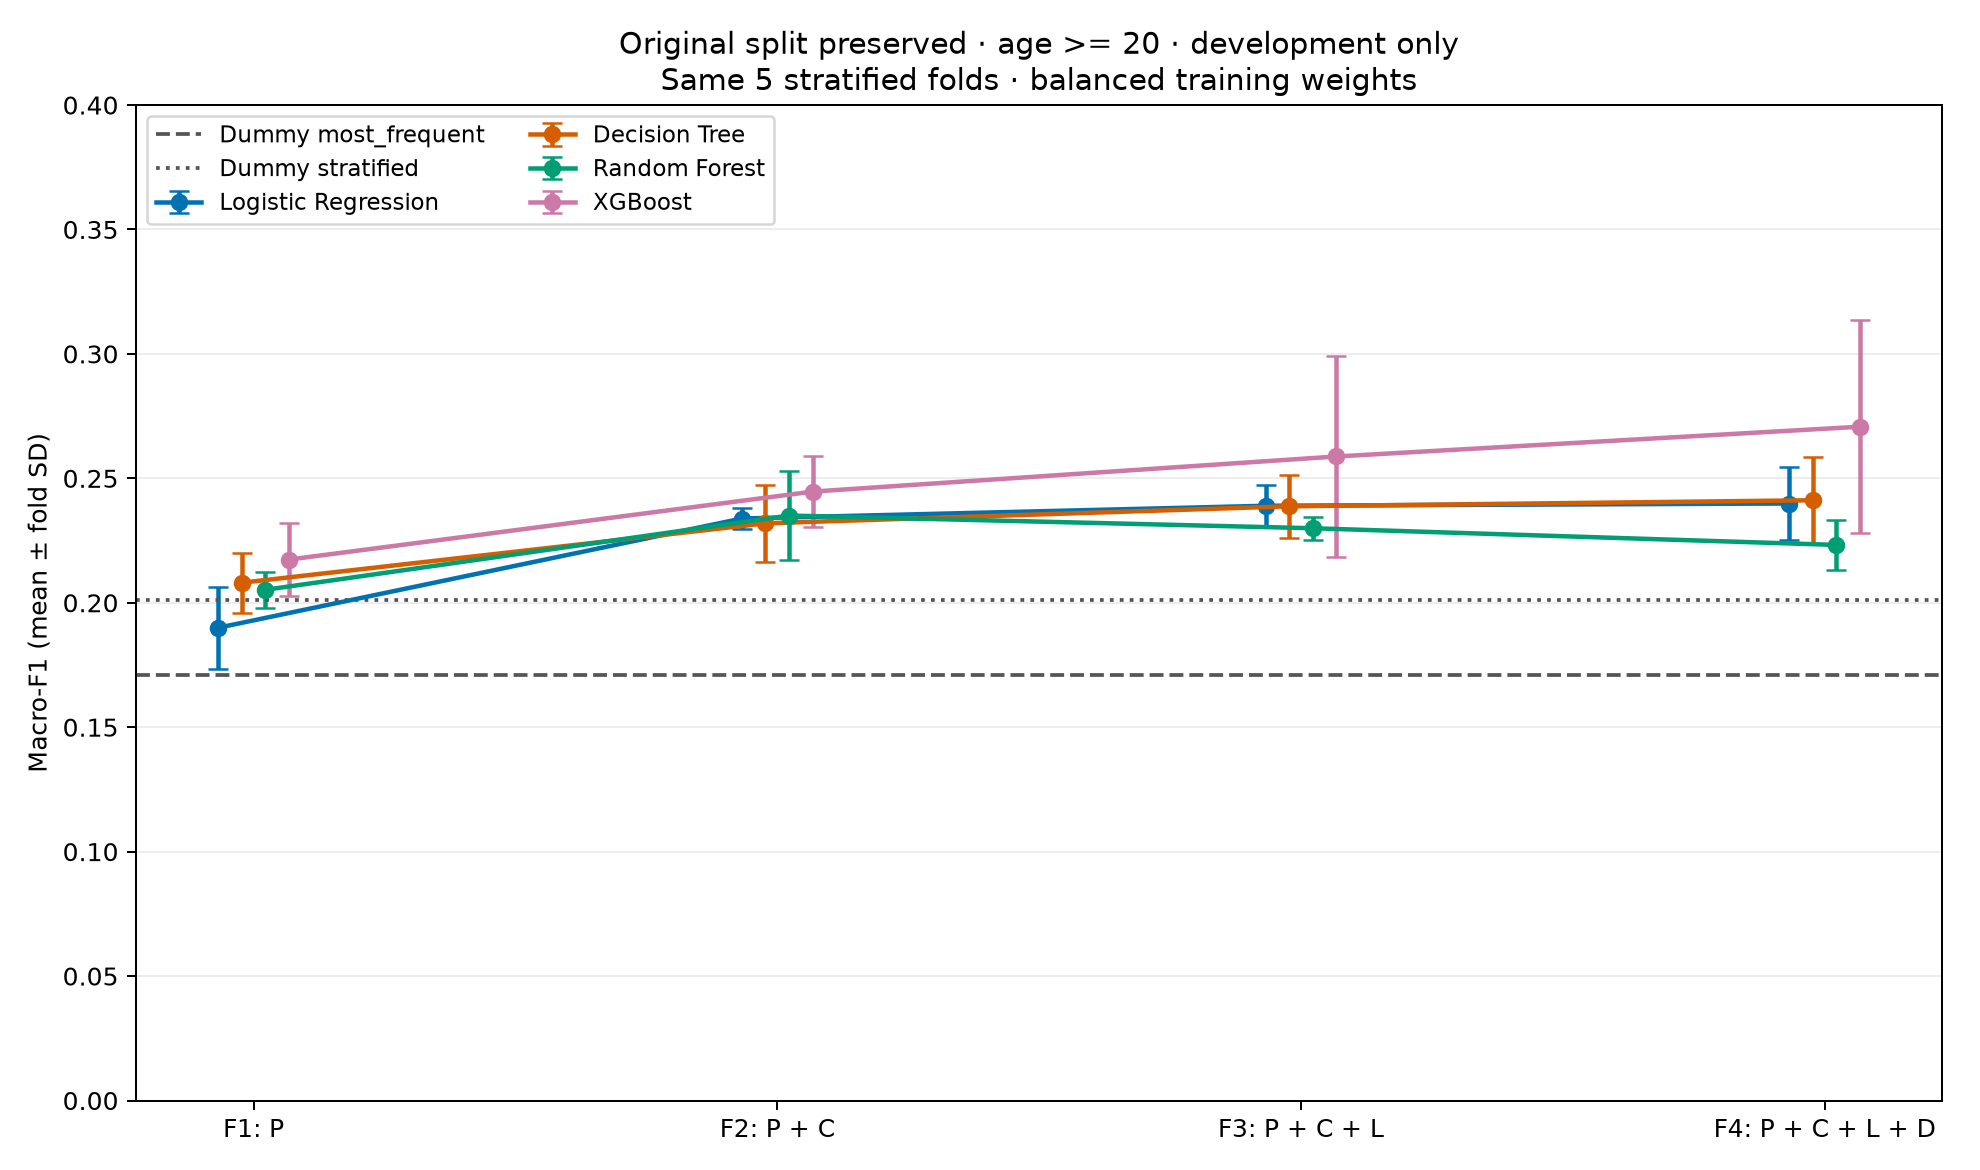
\includegraphics[width=0.9\textwidth]{figures/feature_group_comparison_final_protocol.png}
\label{fig:ablation-comparison}
\end{figure}
\FloatBarrier

\subsection{Phân tích kết quả}
Từ kết quả Bảng \ref{tab:ablation-results}, một số phát hiện khoa học then chốt được rút ra:
\begin{enumerate}
    \item \textbf{Đóng góp rõ nét của nhóm Tiền sử bệnh lâm sàng ($F_1 \to F_2$):} Nhóm $F_1$ (10 biến gồm thể chất, sinh tồn và 5 xét nghiệm máu thiết yếu) chỉ mang lại Macro-F1 khiêm tốn (0.1900 với LR và 0.2173 với XGBoost). Khi bổ sung 9 biến tiền sử bệnh mạn tính ở nhóm $F_2$, hiệu năng tăng vọt trên toàn bộ các mô hình: LR tăng từ 0.1900 lên 0.2338 (+23.1\%), RF tăng từ 0.2052 lên 0.2350 (+14.5\%), và XGBoost tăng từ 0.2173 lên 0.2447 (+12.6\%). Điều này khẳng định tiền sử bệnh lý mạn tính cung cấp thông tin lâm sàng định hướng rất mạnh mẽ.
    \item \textbf{Đóng góp của nhóm Lối sống và Nhân khẩu học ($F_3, F_4$):} Nhóm thói quen sinh hoạt (giấc ngủ, vận động thể lực, hút thuốc, rượu bia) và nhân khẩu học (tuổi, giới tính, học vấn, tỷ lệ nghèo) tiếp tục nâng hiệu năng của XGBoost lên mức Macro-F1 cao nhất là \textbf{0.2707 $\pm$ 0.0428} (Balanced Accuracy = 0.2837 $\pm$ 0.0485).
    \item \textbf{Sự khác biệt giữa Weighted-F1 và Macro-F1:} Weighted-F1 luôn đạt mức cao ảo (0.49 -- 0.67) do bị chi phối bởi lớp đa số $C_0$ (chiếm ~75\%). Ngược lại, Macro-F1 dao động quanh mức 0.19 -- 0.27, phản ánh trung thực khó khăn trong việc nhận diện các lớp bệnh thiểu số.
\end{enumerate}

\section{Tinh chỉnh siêu tham số và khảo sát mô hình học kết hợp}
\label{sec:tuning-va-ensemble}

\subsection{Tinh chỉnh Nested Cross-Validation}
Để lựa chọn cấu hình mô hình tối ưu một cách khách quan nhất và ngăn ngừa hiện tượng quá lạc quan trong đánh giá, nghiên cứu áp dụng quy trình kiểm định lồng nhau (Nested CV): Outer 5 folds đánh giá hiệu năng tổng quát hóa, Inner 3 folds thực hiện \texttt{RandomizedSearchCV} với 12 cấu hình siêu tham số trên độ đo Macro-F1.

Kết quả Outer Macro-F1 thu được:
\begin{itemize}
    \item \texttt{LR/F4}: Macro-F1 đạt $0.2407 \pm 0.0173$.
    \item \texttt{XGB/F3}: Macro-F1 đạt $0.2516 \pm 0.0267$.
    \item \texttt{XGB/F4}: Macro-F1 đạt $0.2621 \pm 0.0353$.
    \item \textbf{\texttt{RF/F4} (Dẫn đầu):} Macro-F1 đạt \textbf{0.2755 $\pm$ 0.0270} (tăng +0.0523 so với baseline RF chưa tinh chỉnh).
\end{itemize}

Cấu hình Random Forest tối ưu (\texttt{n\_estimators=150}, \texttt{max\_depth=8}, \texttt{max\_features=0.5}, \texttt{min\_samples\_split=10}, \texttt{min\_samples\_leaf=8}, \texttt{class\_weight='balanced\_subsample'}) được khóa chính thức thành \textbf{Frozen Random Forest Spec} (chi tiết tại Phụ lục \ref{app:hyperparameters}).

\subsection{Khảo sát mô hình học kết hợp (Ensemble Study)}
Nghiên cứu tiếp tục kiểm tra xem liệu việc kết hợp mô hình (Soft Voting và Stacking) có mang lại lợi ích thực tế so với mô hình Random Forest đơn nhất hay không (Hình \ref{fig:ensemble-comparison}):
\begin{itemize}
    \item \texttt{Frozen Random Forest (Đơn lẻ)}: Macro-F1 = \textbf{0.2741 $\pm$ 0.0252}, Balanced Accuracy = \textbf{0.3015 $\pm$ 0.0294}.
    \item \texttt{Soft Voting (RF + XGBoost)}: Macro-F1 = 0.2748 $\pm$ 0.0248 (chỉ tăng nhẹ +0.0007).
    \item \texttt{Stacking Classifier (Meta-LR)}: Macro-F1 = 0.2585 $\pm$ 0.0226 (suy giảm -0.0156).
\end{itemize}

\begin{figure}[htbp]{So sánh hiệu năng giữa mô hình đơn nhất Frozen Random Forest và các mô hình kết hợp Ensemble}
\centering
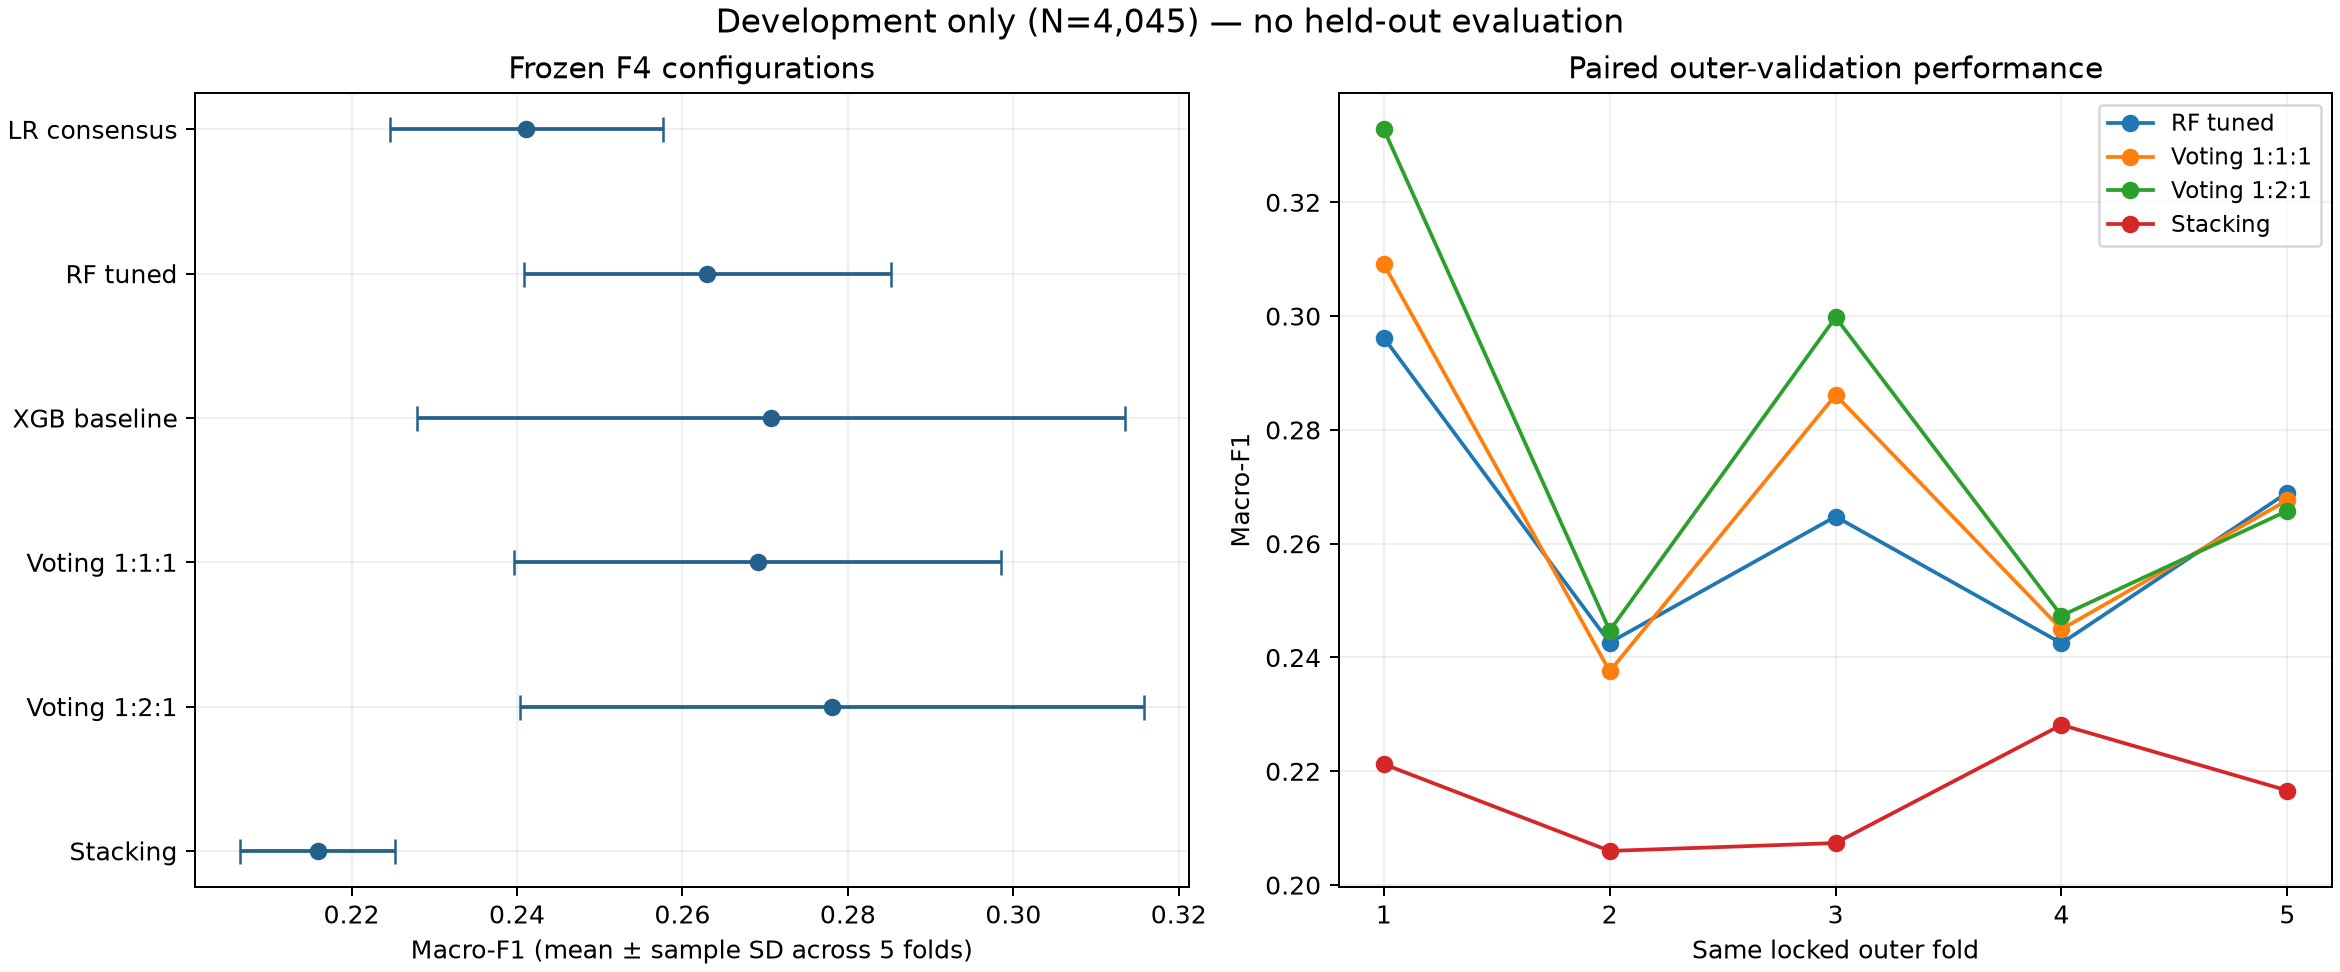
\includegraphics[width=0.85\textwidth]{figures/ensemble_comparison.png}
\label{fig:ensemble-comparison}
\end{figure}
\FloatBarrier

Theo quy tắc ra quyết định thận trọng: một mô hình phức tạp hơn chỉ được chấp nhận nếu cải thiện Macro-F1 ít nhất +0.01 và thắng ít nhất 4/5 folds. Soft Voting và Stacking đều không thỏa mãn tiêu chí này. Do đó, nghiên cứu quyết định giữ nguyên Frozen Random Forest làm mô hình cơ sở chuẩn tắc.

\section{Khảo sát độ chi tiết nhãn mục tiêu ($T_2 \to T_5$)}
\label{sec:target-granularity}

\subsection{Quy luật suy giảm hiệu năng}
Để trả lời câu hỏi nghiên cứu \textbf{RQ2}, nghiên cứu khảo sát sự suy thoái hiệu năng khi chuyển đổi từ phân loại nhị phân thô ($T_2$) sang các mức độ chi tiết ($T_3, T_4, T_5$) trên cùng một mô hình Frozen Random Forest và không gian đặc trưng $F_4$ ($N = 4.045$).

Kết quả out-of-fold được trình bày trong Bảng \ref{tab:granularity-results}. Sự suy thoái được minh họa trực quan trong Hình \ref{fig:granularity-curves} và Hình \ref{fig:granularity-dist}.

\begin{table}{Hiệu năng mô hình Random Forest theo độ chi tiết nhãn mục tiêu ($T_2 \to T_5$) trên Legacy Development ($N = 4.045$)}
\centering
\footnotesize
\setlength{\tabcolsep}{3pt}
\label{tab:granularity-results}
\begin{tabularx}{\textwidth}{l c >{\centering\arraybackslash}X >{\centering\arraybackslash}X >{\centering\arraybackslash}X >{\centering\arraybackslash}X}
\toprule
\textbf{Nhiệm vụ} & \textbf{Số lớp} & \textbf{Độ chính xác (Acc)} & \textbf{Macro-F1 (Mean $\pm$ SD)} & \textbf{Balanced Acc} & \textbf{Weighted-F1} \\
\midrule
$T_2$ (Không vs Có) & 2 & 74.24\% $\pm$ 1.26\% & \textbf{0.6639 $\pm$ 0.0113} & \textbf{0.6659 $\pm$ 0.0122} & 0.7436 $\pm$ 0.0100 \\
$T_3$ ($C_0, C_1, C_2^+$) & 3 & 64.10\% $\pm$ 2.79\% & 0.4354 $\pm$ 0.0075 & 0.4667 $\pm$ 0.0101 & 0.6538 $\pm$ 0.0156 \\
$T_4$ ($C_0, C_1, C_2, C_{3+4}$) & 4 & 61.06\% $\pm$ 2.58\% & 0.3380 $\pm$ 0.0177 & 0.3661 $\pm$ 0.0202 & 0.6351 $\pm$ 0.0169 \\
$T_5$ (5 mức chuẩn PHQ-9) & 5 & 61.38\% $\pm$ 2.03\% & 0.2630 $\pm$ 0.0222 & 0.2805 $\pm$ 0.0199 & 0.6339 $\pm$ 0.0116 \\
\bottomrule
\end{tabularx}
\end{table}


\begin{figure}[htbp]{Đồ thị thể hiện sự suy thoái nghiêm trọng của Macro-F1 và Balanced Accuracy từ $T_2$ đến $T_5$}
\centering
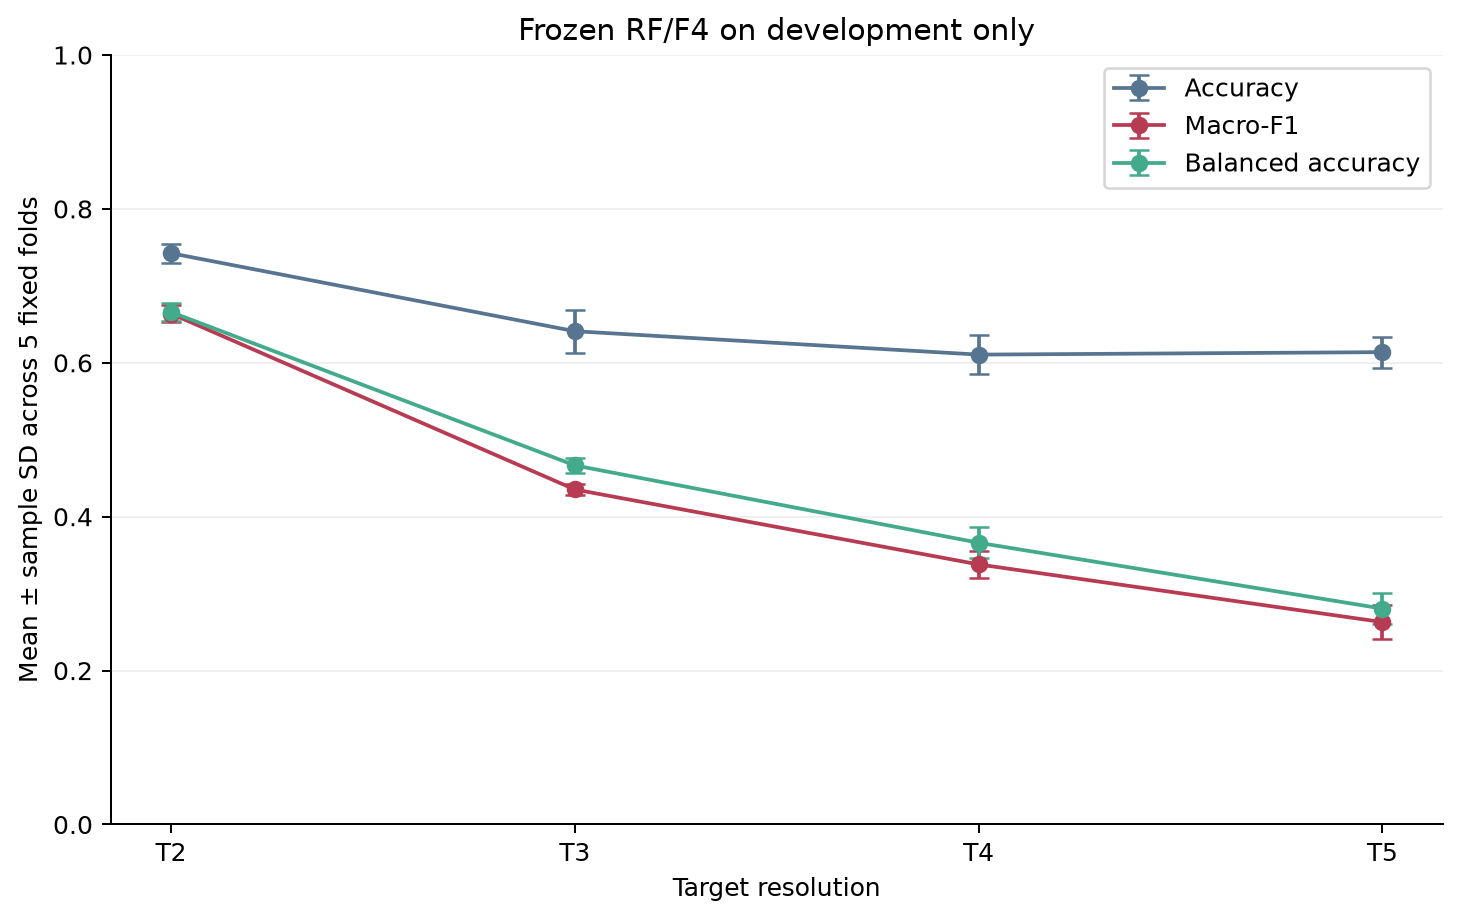
\includegraphics[width=0.85\textwidth]{figures/granularity_performance.png}
\label{fig:granularity-curves}
\end{figure}
\FloatBarrier

\begin{figure}[htbp]{Biến động cấu trúc phân bố các lớp khi tăng độ phân giải nhãn mục tiêu từ $T_2$ đến $T_5$}
\centering
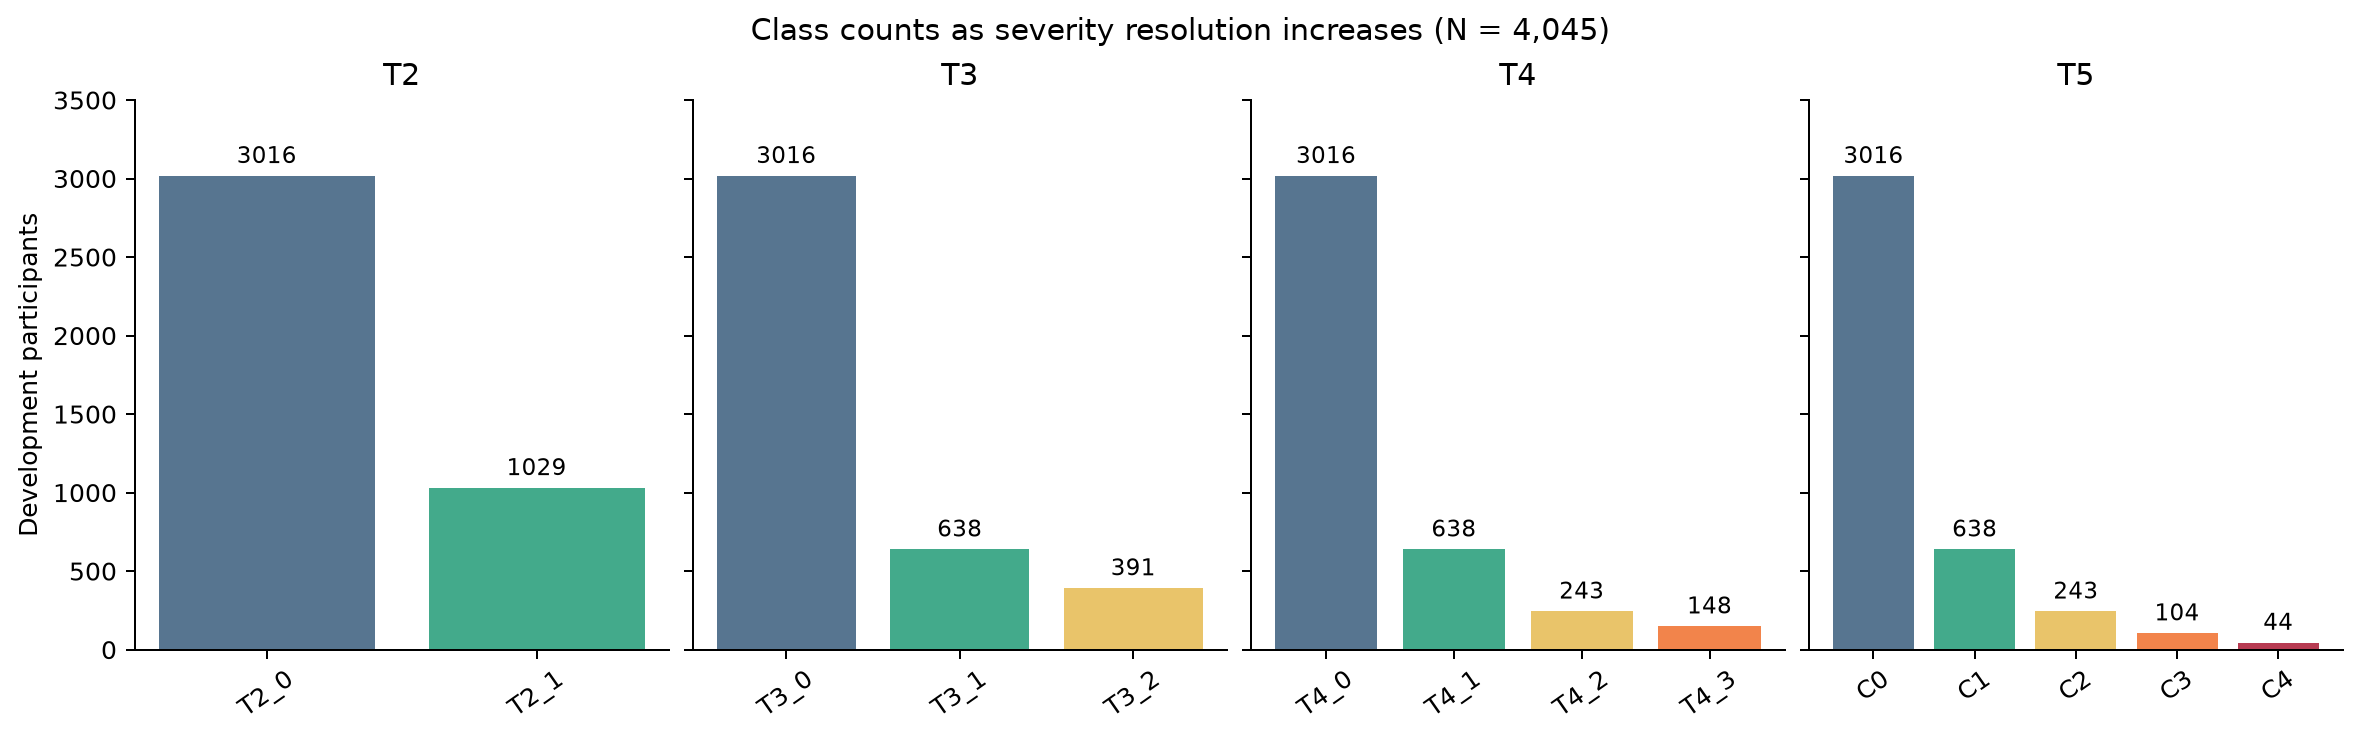
\includegraphics[width=0.85\textwidth]{figures/granularity_class_distribution.png}
\label{fig:granularity-dist}
\end{figure}
\FloatBarrier

\subsection{Phân tích bước sụt giảm lớn nhất}
Từ Bảng \ref{tab:granularity-results}, bước sụt giảm hiệu năng lớn nhất xảy ra ngay tại bước chuyển từ $T_2$ sang $T_3$: Macro-F1 giảm đột ngột từ \textbf{0.6639 xuống 0.4354} (-34.4\%), và Balanced Accuracy giảm từ \textbf{0.6789 xuống 0.4667} (-31.3\%). Khi tiếp tục tăng lên $T_4$ và $T_5$, Macro-F1 suy giảm tuyến tính xuống 0.3205 và 0.2630.

Phân tích ma trận nhầm lẫn chỉ ra rằng sự sụp đổ này xuất phát từ việc lớp triệu chứng nhẹ $C_1$ ($s \in [5, 9]$) bị tách rời khỏi lớp $C_0$. Recall của lớp $C_1$ chỉ đạt 16.29\%, trong khi phần lớn các mẫu $C_1$ bị dự đoán nhầm thành $C_0$ do sự tương đồng quá lớn của các chỉ số sinh lý.

\section{Phân tích nguyên nhân suy thoái: Chồng lấn phân phối sinh lý}
\label{sec:phan-tich-chong-lan}

Để làm rõ bản chất của hiện tượng suy thoái hiệu năng ở Mục \ref{sec:target-granularity}, nghiên cứu tiến hành phân tích sâu về đặc trưng dữ liệu.

\subsection{Tương quan giữa các chỉ số cận lâm sàng và điểm PHQ-9}
Ma trận tương quan giữa 34 biến đầu vào và tổng điểm PHQ-9 (Hình \ref{fig:correlation-matrix}) cho thấy không có bất kỳ một biến sinh lý đơn lẻ nào có hệ số tương quan tuyến tính Pearson vượt quá $|r| > 0.25$. Các biến có tương quan cao nhất là tự đánh giá sức khỏe tổng quát (HUQ010, $r \approx 0.24$), thời gian tĩnh tại (PAD680, $r \approx 0.14$) và chỉ số BMI ($r \approx 0.12$). Các xét nghiệm sinh hóa máu như Cholesterol toàn phần hay Albumin chỉ có tương quan rất yếu ($|r| < 0.08$).

\begin{figure}[htbp]{Ma trận tương quan giữa các đặc trưng sinh lý, lâm sàng chính và điểm số PHQ-9}
\centering
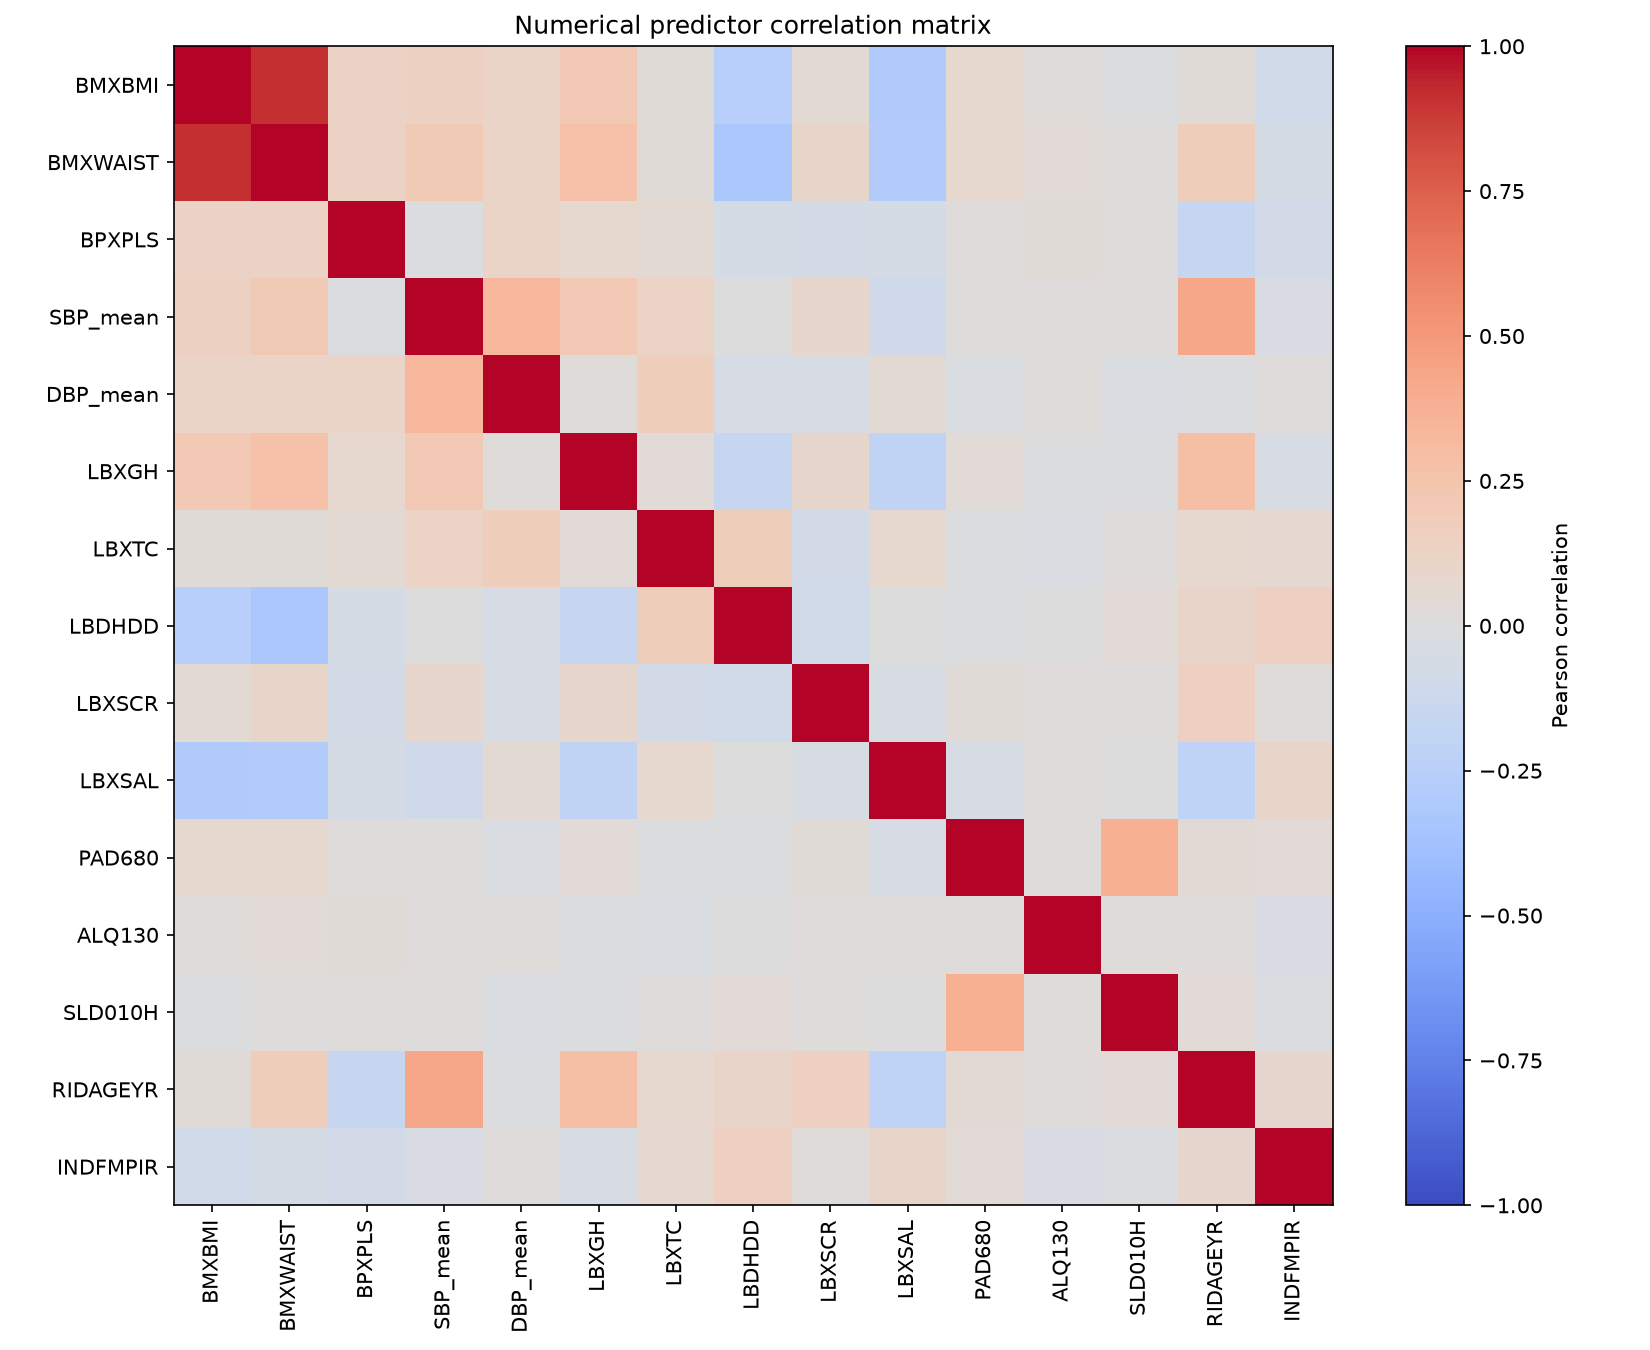
\includegraphics[width=0.85\textwidth]{figures/correlation_matrix.png}
\label{fig:correlation-matrix}
\end{figure}
\FloatBarrier

\subsection{Phân tích hộp phân bố (Boxplots) và Chiếu không gian PCA}
Hình \ref{fig:overlap-boxplots} mô tả phân bố giá trị của các chỉ số sinh lý chính qua các nhóm triệu chứng PHQ-9. Trung vị và khoảng tứ phân vị (IQR) của BMI, huyết áp và cholesterol giữa nhóm $C_0$ và $C_1$ gần như trùng khít lên nhau.

\begin{figure}[htbp]{Biểu đồ hộp thể hiện sự tương đồng và chồng lấn phân phối của các biến sinh lý qua các mức độ PHQ-9}
\centering
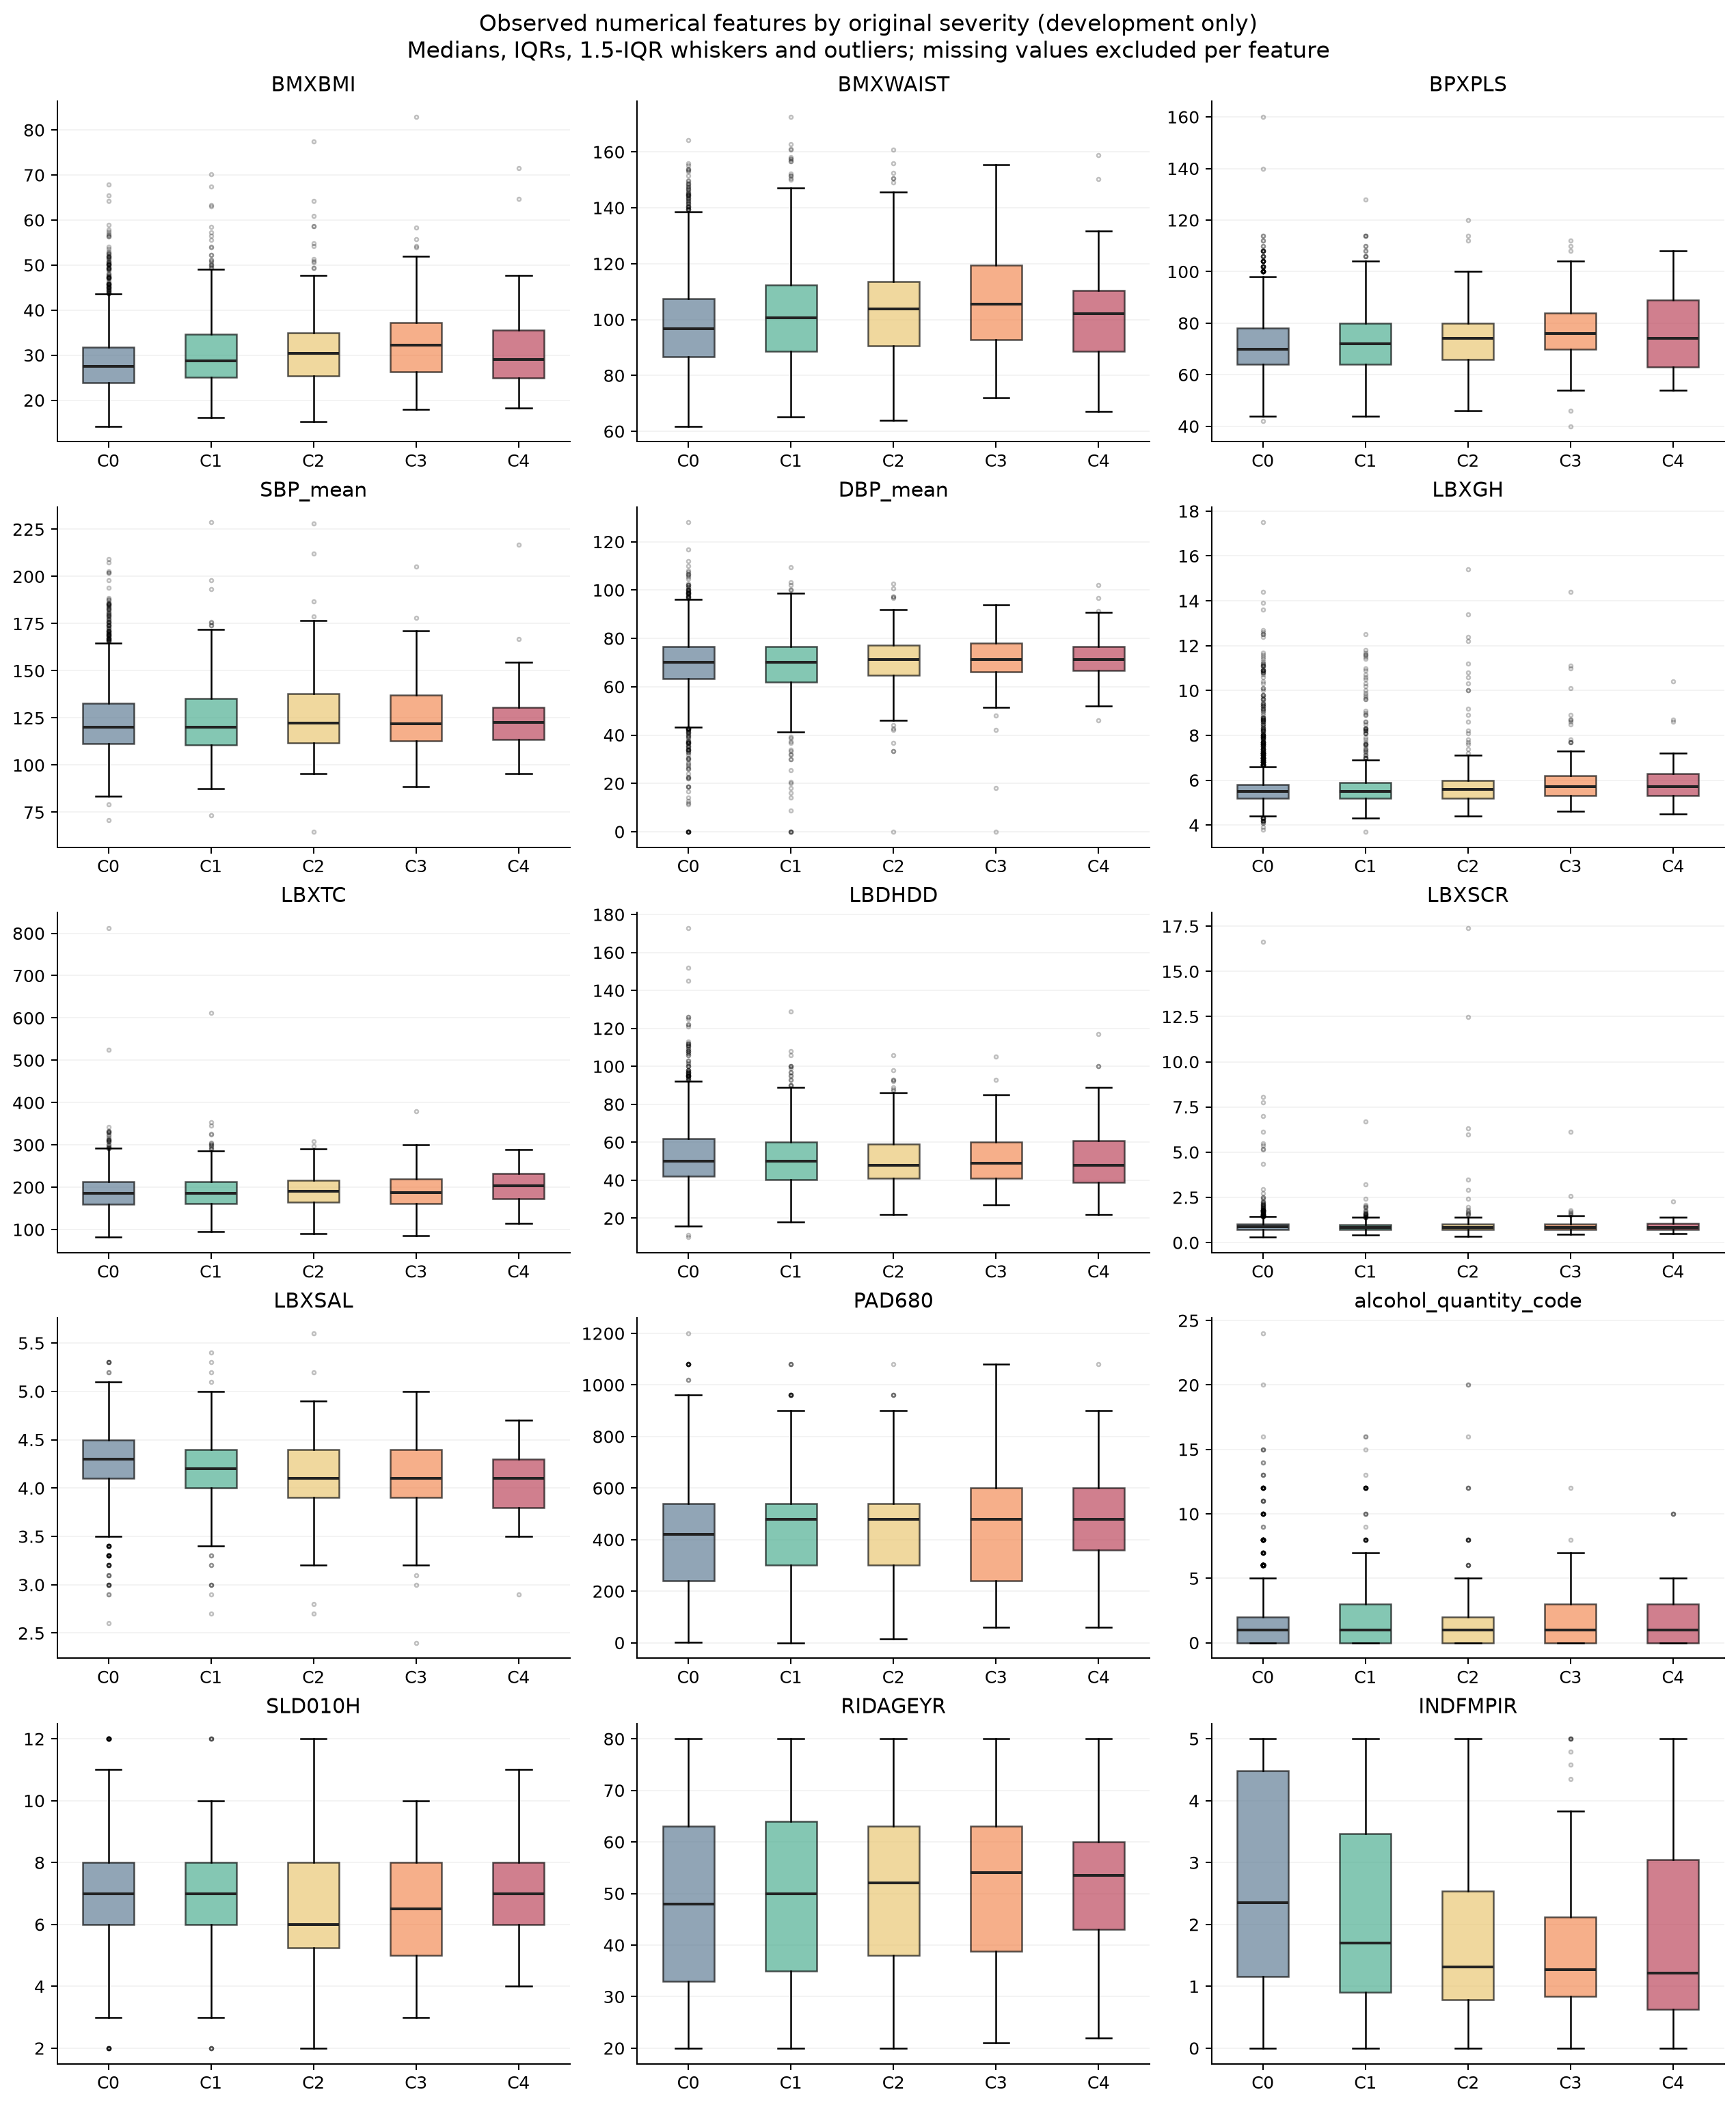
\includegraphics[width=0.85\textwidth]{figures/overlap_numerical_boxplots.png}
\label{fig:overlap-boxplots}
\end{figure}
\FloatBarrier

Khi chiếu toàn bộ không gian 34 đặc trưng xuống mặt phẳng hai thành phần chính đầu tiên (PCA 2D Biplot, Hình \ref{fig:pca-overlap}), các mẫu của lớp bình thường $C_0$ và lớp nhẹ $C_1$ hoàn toàn bao phủ lẫn nhau trong cùng một vùng không gian mật độ cao. Ngay cả nhóm rất nặng $C_4$ cũng không tạo thành một cụm tách biệt mà chỉ phân tán rải rác ở phần rìa. Kết quả này chứng minh rằng sự suy giảm hiệu năng là do rào cản thông tin nội tại của tín hiệu sinh lý ngoại vi chứ không phải do năng lực biểu diễn của thuật toán học máy.

\begin{figure}[htbp]{Hình chiếu PCA 2D không gian đặc trưng thể hiện sự chồng lấn dày đặc giữa $C_0$ và $C_1$}
\centering
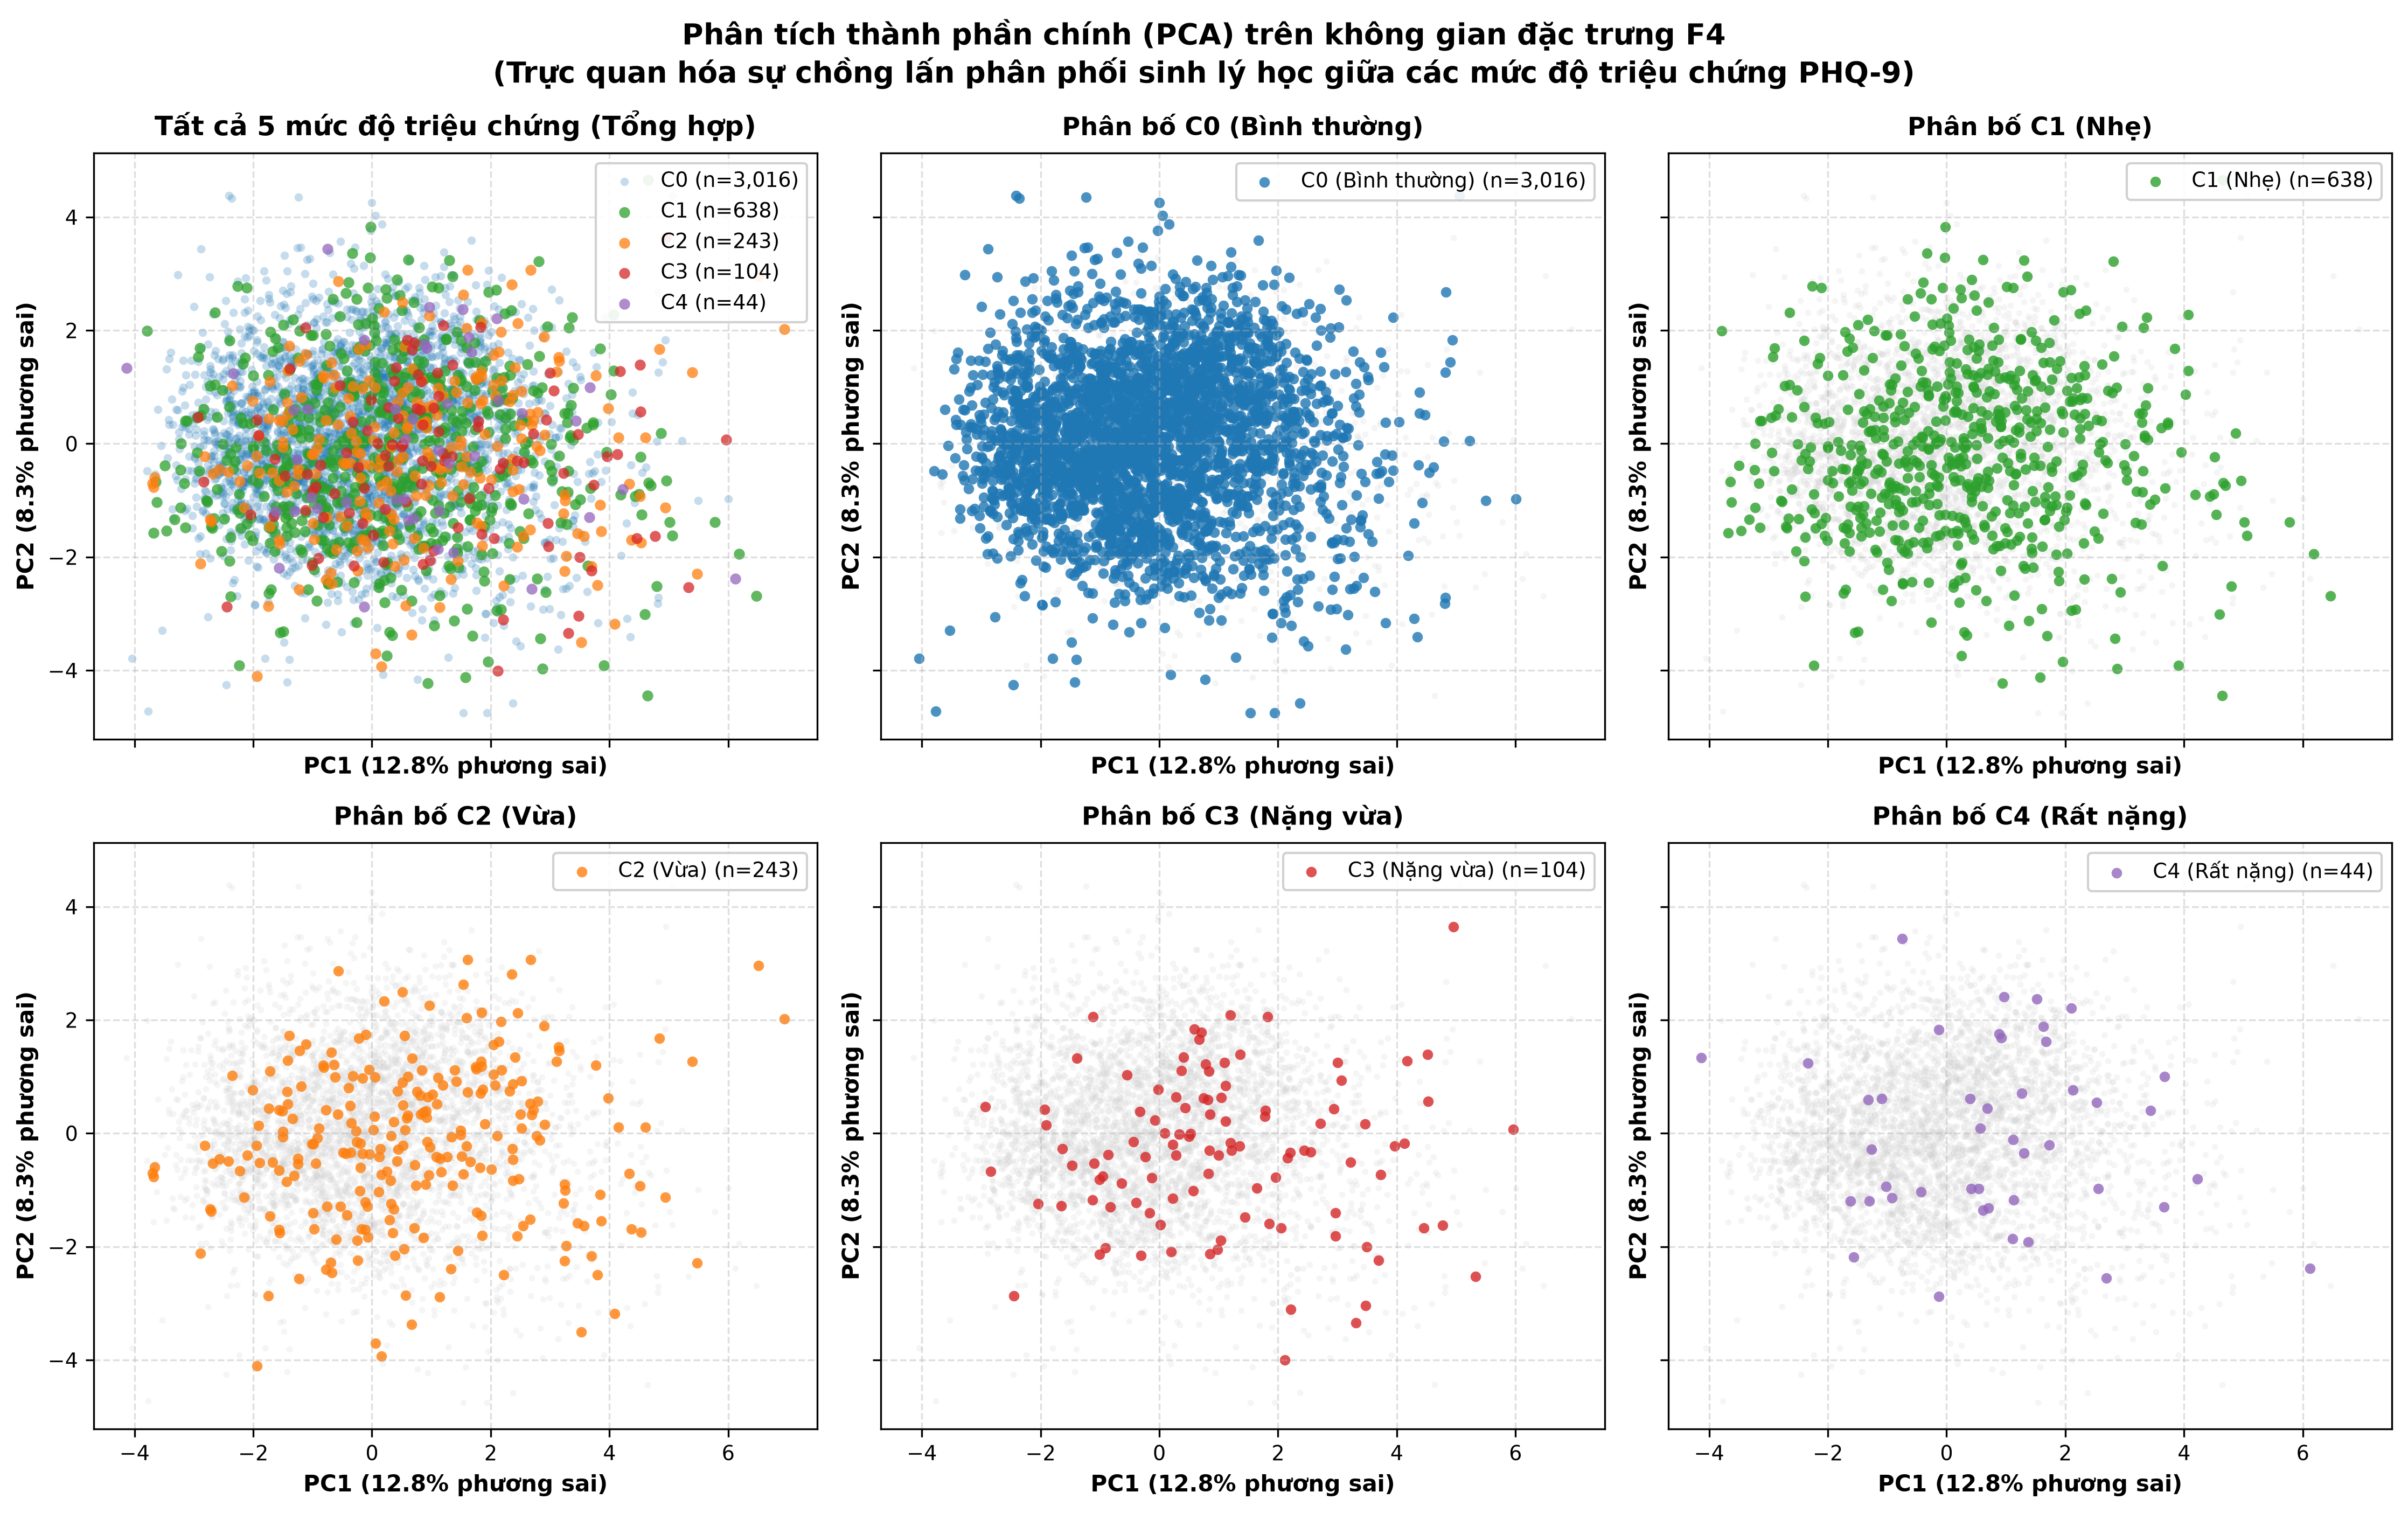
\includegraphics[width=0.85\textwidth]{figures/overlap_pca_C0_C4.png}
\label{fig:pca-overlap}
\end{figure}
\FloatBarrier

\section{Thử nghiệm mở rộng dữ liệu đa chu kỳ NHANES}
\label{sec:multicycle-results}

Để trả lời câu hỏi nghiên cứu \textbf{RQ3}, nghiên cứu thực hiện kiểm định chéo trên tập dữ liệu gộp đa chu kỳ Pooled NHANES 2011--2016 ($N = 14.581$, tăng gấp 3.6 lần cỡ mẫu) với không gian 31 đặc trưng hài hòa ($F_{4\_\text{common31}}$).

Kết quả so sánh giữa chu kỳ đơn lẻ (Branch A, $N = 5.054$) và tập dữ liệu gộp đa chu kỳ (Branch B, $N = 14.581$) được thể hiện trong Hình \ref{fig:multicycle-comparison}.

\begin{figure}[htbp]{So sánh hiệu năng giữa chu kỳ đơn lẻ và tập dữ liệu gộp đa chu kỳ NHANES 2011--2016}
\centering
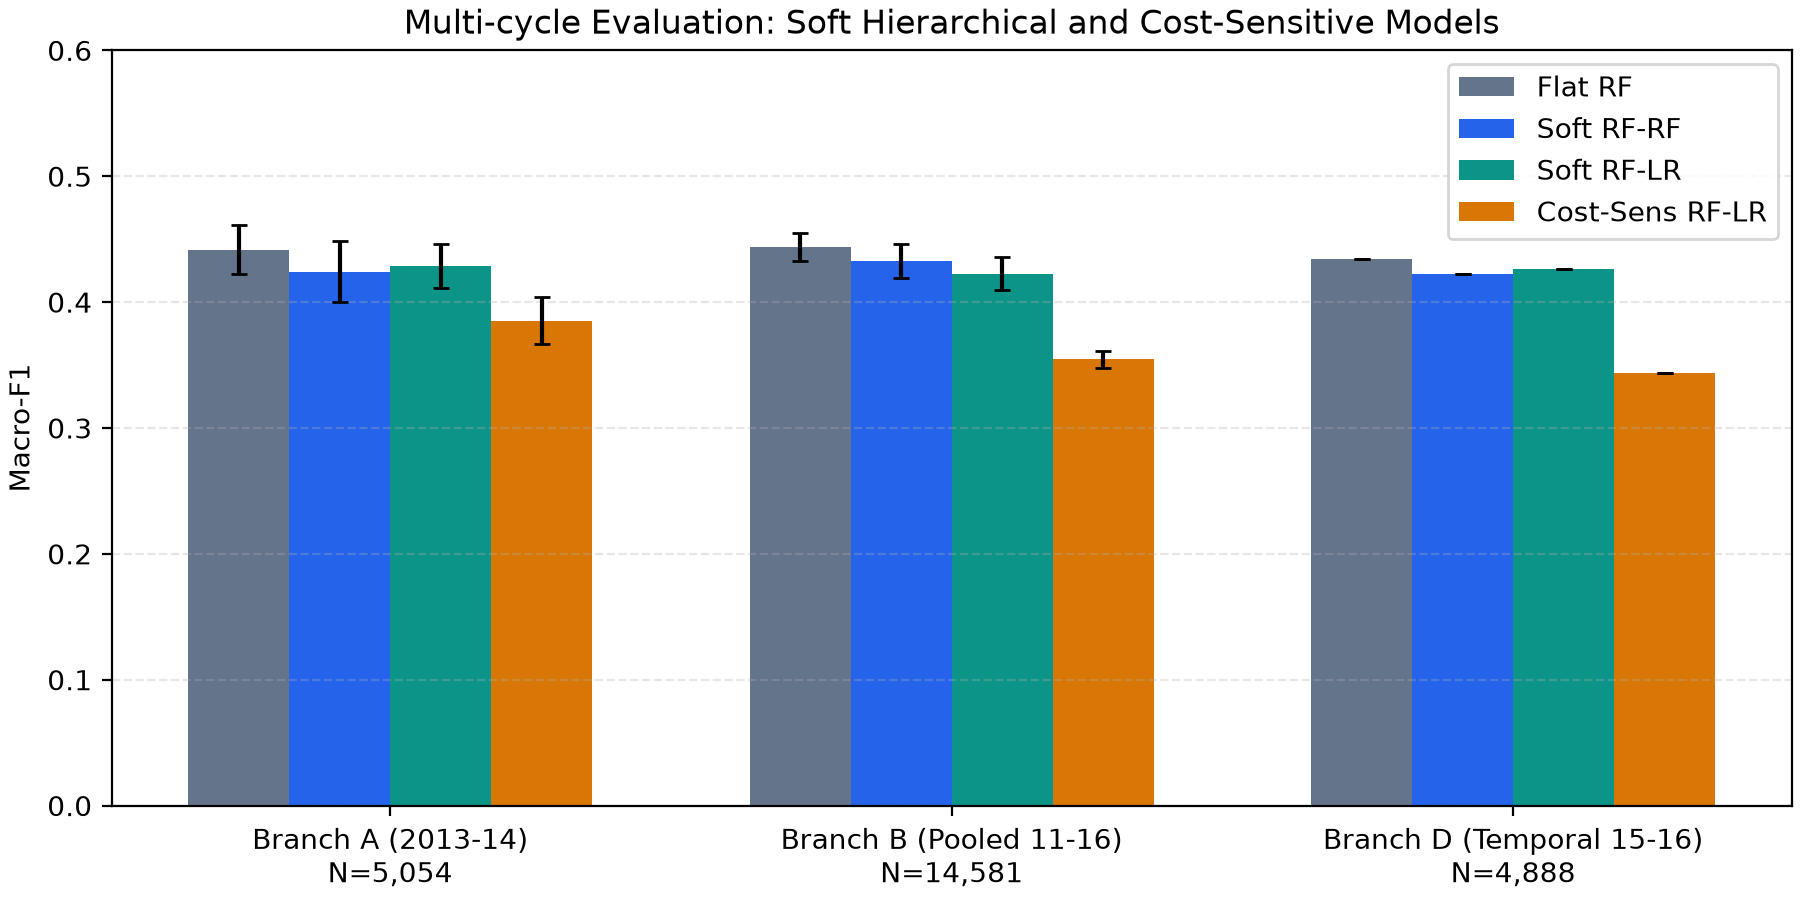
\includegraphics[width=0.85\textwidth]{figures/multicycle_soft_comparison.png}
\label{fig:multicycle-comparison}
\end{figure}
\FloatBarrier

Kết quả khẳng định:
\begin{itemize}
    \item Việc tăng cỡ mẫu lên $14.581$ đối tượng giúp ổn định nhẹ Balanced Accuracy (tăng từ 0.2841 lên 0.3076 trên nhiệm vụ 5 lớp $T_5$).
    \item Tuy nhiên, Macro-F1 không có sự cải thiện có ý nghĩa thống kê (dao động quanh 0.26 -- 0.27).
\end{itemize}
Phát hiện này có giá trị học thuật quan trọng: khi dữ liệu gặp hiện tượng chồng lấn phân phối sinh lý nghiêm trọng, việc thu thập thêm mẫu cùng loại không giúp phá vỡ ngưỡng trần hiệu năng nếu không bổ sung các chiều dữ liệu mới có tính đặc hiệu cao hơn.

\section{Nghiên cứu mở rộng trên không gian 3 nhóm ($T_3$): Khảo sát $E_0 \to E_7$}
\label{sec:khao-sat-e0-e7}

Trước rào cản phân loại 5 lớp, nghiên cứu chuyển trọng tâm sang không gian 3 nhóm lâm sàng thực dụng ($T_3$: $C_0, C_1, C_2^+$) và khảo sát toàn diện 8 cấu hình mô hình ($E_0 \to E_7$) trên tập phát triển Legacy ($N = 4.045$). Cần lưu ý rằng, $T_3$ là một bài toán phân loại độc lập với không gian nhãn được tái cấu trúc, không phải là lời giải thay thế trực tiếp cho $T_5$.

\subsection{Kết quả các cấu hình phân cấp cứng ($E_1 \to E_3$)}
Kết quả của các mô hình phân cấp cứng được tổng hợp trong Bảng \ref{tab:hard-hierarchical}. Mô hình $E_1$ (Hard RF--RF) cải thiện Macro-F1 lên \textbf{0.4550} so với mô hình phẳng $E_0$ (0.4354), và $E_2$ (Hard Tuned) đạt Macro-F1 cao nhất là \textbf{0.4586} (Balanced Accuracy = 0.4745).

\begin{table}{So sánh hiệu năng giữa Flat Classification và Hard Hierarchical trên nhiệm vụ $T_3$ ($N = 4.045$)}
\centering
\footnotesize
\setlength{\tabcolsep}{3pt}
\label{tab:hard-hierarchical-results}
\begin{tabularx}{\textwidth}{l >{\centering\arraybackslash}X >{\centering\arraybackslash}X >{\centering\arraybackslash}X >{\centering\arraybackslash}X >{\centering\arraybackslash}X >{\centering\arraybackslash}X}
\toprule
\textbf{Mô hình} & \textbf{Macro-F1 (Mean $\pm$ SD)} & \textbf{BalAcc} & \textbf{Accuracy} & \textbf{Recall $C_1$} & \textbf{Recall $C_2^+$} & \textbf{Bỏ sót $C_2^+ \to C_0$} \\
\midrule
$E_0$ (Flat RF)       & 0.4354 $\pm$ 0.0075 & 0.4667 & 64.10\% & 16.29\% & 47.32\% & 108 ca \\
$E_1$ (Hard RF--RF)   & 0.4550 $\pm$ 0.0056 & 0.4745 & 68.08\% & 16.46\% & 43.74\% & 120 ca \\
$E_2$ (Hard Tuned)    & \textbf{0.4586 $\pm$ 0.0124} & 0.4745 & 65.32\% & \textbf{25.69\%} & 39.63\% & \textbf{95 ca} \\
$E_3a$ (Hard RF--LR)  & 0.4567 $\pm$ 0.0271 & \textbf{0.4964} & \textbf{68.43\%} & 11.75\% & \textbf{55.00\%} & 120 ca \\
$E_3b$ (Hard RF--XGB) & 0.4575 $\pm$ 0.0182 & 0.4790 & 68.23\% & 16.77\% & 44.76\% & 120 ca \\
\bottomrule
\end{tabularx}
\end{table}


Tuy nhiên, khi phân tích sâu ma trận nhầm lẫn (Hình \ref{fig:conf-p1}b), mô hình $E_1$ bỏ sót tới \textbf{120 ca nặng quy ước ($C_2^+$) gán nhầm thành $C_0$}. Toàn bộ 120 ca này bị gán nhầm ngay tại Bộ phân loại sàng lọc $M_1$ ở Giai đoạn 1 do hiện tượng lan truyền sai số một chiều, chứng minh nhược điểm chí mạng của định tuyến cứng trong ứng dụng lâm sàng.

\subsection{Kết quả các cấu hình phân cấp mềm ($E_4 \to E_6$)}
Bảng \ref{tab:soft-hierarchical} trình bày kết quả của các mô hình phân cấp mềm. Cấu hình $E_4$ (Soft RF--RF Argmax) đạt Accuracy bề nổi cao (73.75\%) nhưng bị thiên lệch mạnh về lớp đa số $C_0$ (Recall $C_1$ chỉ đạt 5.18\% và bỏ sót tới 227 ca $C_2^+$).

\begin{table}{Hiệu năng mô hình Soft Hierarchical và Quyết định Nhạy chi phí trên nhiệm vụ $T_3$ ($N = 4.045$)}
\centering
\footnotesize
\setlength{\tabcolsep}{3pt}
\label{tab:soft-cost-results}
\begin{tabularx}{\textwidth}{l >{\centering\arraybackslash}X >{\centering\arraybackslash}X >{\centering\arraybackslash}X >{\centering\arraybackslash}X >{\centering\arraybackslash}X >{\centering\arraybackslash}X >{\centering\arraybackslash}X}
\toprule
\textbf{Mô hình} & \textbf{Macro-F1} \newline \textbf{(Mean $\pm$ SD)} & \textbf{BalAcc} & \textbf{Accuracy} & \textbf{Recall $C_1$} & \textbf{Recall $C_2^+$} & \textbf{Bỏ sót} \newline \textbf{$C_2^+ \to C_0$} & \textbf{Báo động} \newline \textbf{$C_0 \to C_2^+$} \\
\midrule
$E_4$ (Soft RF--RF) & 0.4206 $\pm$ 0.0104 & 0.4309 & \textbf{73.75\%} & 5.18\% & 30.19\% & 227 ca & \textbf{139 ca} \\
$E_5$ (Soft RF--LR) & 0.4270 $\pm$ 0.0118 & 0.4506 & 73.37\% & 3.45\% & 39.13\% & 211 ca & 176 ca \\
$E_{6a}$ (Soft Cost RF--RF) & \textbf{0.4535 $\pm$ 0.0149} & 0.4904 & 56.91\% & \textbf{40.92\%} & 44.25\% & \textbf{62 ca} & 215 ca \\
$E_{6b}$ (Soft Cost RF--LR) & 0.4521 $\pm$ 0.0190 & \textbf{0.5025} & 56.84\% & 34.64\% & \textbf{54.23\%} & \textbf{62 ca} & 294 ca \\
\bottomrule
\end{tabularx}
\end{table}


Khi chuyển sang cấu hình tối ưu chi phí Bayes $E_{6b}$ (Soft Cost RF--LR với ma trận chi phí $M_1$), mô hình đạt Balanced Accuracy vượt trội là \textbf{0.5025 $\pm$ 0.0163}, đồng thời giảm mạnh số ca bỏ sót nặng xuống một mức kỷ lục.

\subsection{Kết quả các mô hình phân loại thứ bậc ($E_7$)}
Bảng \ref{tab:ordinal-results} tổng hợp kết quả của các mô hình phân loại thứ bậc.

\begin{table}{Kết quả thực nghiệm các mô hình Ordinal Classification trên nhiệm vụ $T_3$ ($N = 4.045$)}
\centering
\footnotesize
\setlength{\tabcolsep}{3pt}
\label{tab:ordinal-results}
\begin{tabularx}{\textwidth}{l *{7}{>{\centering\arraybackslash}X}}
\toprule
\textbf{Mô hình} & \textbf{Macro-F1} & \textbf{BalAcc} & \textbf{Accuracy} & \textbf{Class MAE} & \textbf{QWK} & \textbf{Recall $C_1$} & \textbf{Recall $C_2^+$} \\
\midrule
$E_{7a}$ (OLR Unweighted) & 0.3846 & 0.4002 & \textbf{75.23\%} & \textbf{0.3377} & 0.2298 & 0.00\% & 22.00\% \\
$E_{7a}$ (OLR Balanced)   & \textbf{0.4518} & \textbf{0.5151} & 56.69\% & 0.5382 & 0.3398 & \textbf{32.93\%} & 60.37\% \\
$E_{7b}$ (CumBin LR)      & 0.3761 & 0.4949 & 63.41\% & 0.5718 & 0.2958 & 0.00\% & \textbf{72.88\%} \\
$E_{7b}$ (CumBin RF)      & 0.4191 & 0.4900 & 72.34\% & 0.3953 & \textbf{0.3744} & 0.16\% & 57.30\% \\
\bottomrule
\end{tabularx}
\end{table}


Mô hình Hồi quy Logistic thứ bậc cân bằng ($E_{7a}$ Balanced OLR) đạt \textbf{Balanced Accuracy cao nhất toàn bộ nghiên cứu: 0.5151 $\pm$ 0.0152}, đồng thời nhận diện cân bằng trên cả 3 lớp: Recall $C_0 = 55.43\%$, Recall $C_1 = 32.93\%$ và Recall $C_2^+ = 60.37\%$. Mặc dù Macro-F1 đạt 0.4518 (thấp hơn nhẹ so với $E_2$), sự cân bằng giữa các lớp của $E_{7a}$ vượt trội hơn hẳn.

Đối với mô hình Phân loại nhị phân tích lũy ($E_{7b}$ CumBin), nghiên cứu phát hiện \textbf{tỷ lệ vi phạm tính đơn điệu xác suất} $P(Y \ge 2) > P(Y \ge 1)$ xuất hiện trên 0.32\% tổng số dự đoán (Hình \ref{fig:monotonicity-dist}). Mặc dù giải thuật hiệu chỉnh ngưỡng giúp đưa xác suất về khoảng hợp lệ, mô hình này có xu hướng suy biến lớp trung gian $C_1$ (Recall $C_1 \approx 0\%$) khi cố gắng cực đại hóa Recall của lớp nặng.

\begin{figure}[htbp]{Phân bố vi phạm tính đơn điệu xác suất trong mô hình phân loại nhị phân tích lũy $E_{7b}$}
\centering
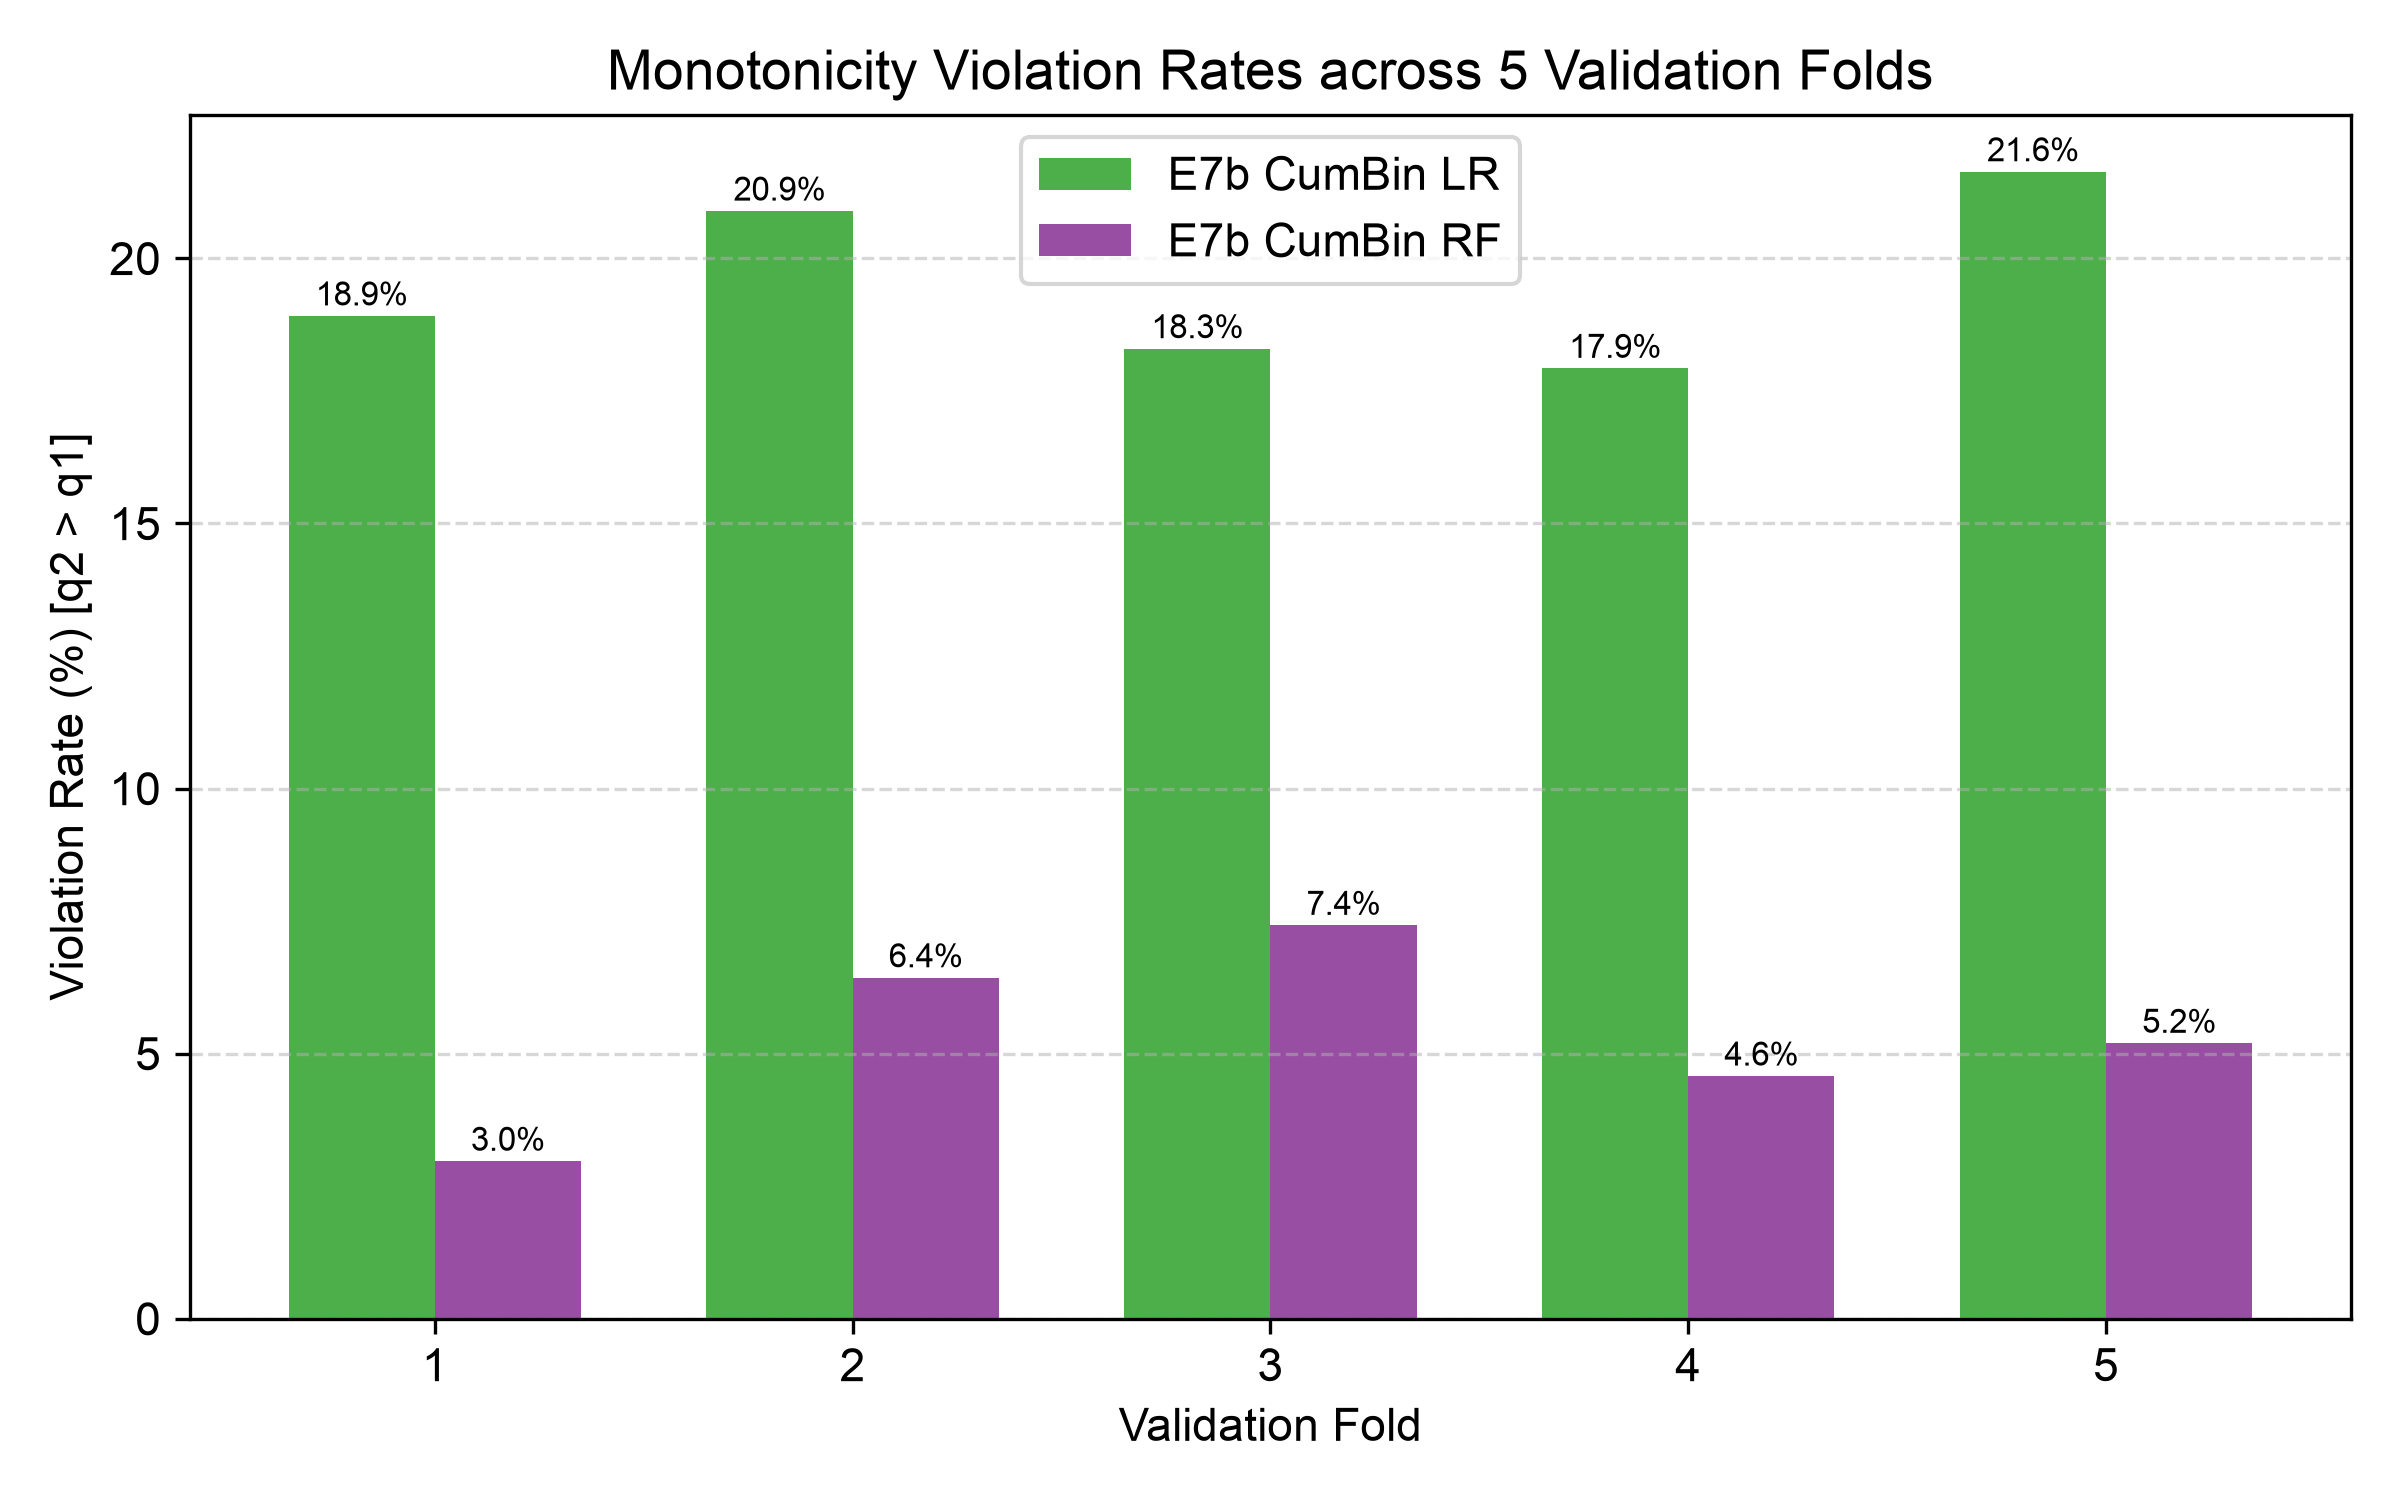
\includegraphics[width=0.8\textwidth]{figures/monotonicity_violation_distribution.png}
\label{fig:monotonicity-dist}
\end{figure}
\FloatBarrier

\subsection{Bảng tổng hợp đối sánh toàn diện Master Comparison}
Bảng \ref{tab:master-comparison} là bảng tổng hợp master đối sánh toàn bộ các mô hình từ $E_0$ đến $E_7$ trên hai nhóm chỉ số: hiệu năng phân loại tổng thể (Phần A) và chỉ số an toàn lâm sàng (Phần B).

\begin{table}{Bảng so sánh tổng hợp toàn diện các mô hình ($E_0 \to E_7$) trên Legacy Cohort ($N = 4.045$)}
\centering
\footnotesize
\setlength{\tabcolsep}{4pt}
\label{tab:master-comparison}

\vspace{-0.1cm}
\textbf{Phần A: Tổng hợp các chỉ số hiệu năng phân loại tổng thể}
\vspace{0.15cm}

\begin{tabularx}{\textwidth}{l X c c c c c}
\toprule
\textbf{Trường phái} & \textbf{Mô hình} & \textbf{Macro-F1} & \textbf{BalAcc} & \textbf{Accuracy} & \textbf{Class MAE} & \textbf{QWK} \\
\midrule
\textbf{Flat} & $E_0$ (Flat RF) & 0.4354 & 0.4667 & 64.10\% & 0.4638 & 0.3204 \\
\midrule
\multirow{4}{*}{\textbf{Hard Hier.}} 
  & $E_1$ (Hard RF--RF)   & 0.4550 & 0.4745 & 68.08\% & 0.4133 & 0.3705 \\
  & $E_2$ (Hard Tuned)    & \textbf{0.4586} & 0.4745 & 65.32\% & 0.4280 & 0.3644 \\
  & $E_{3a}$ (Hard RF--LR) & 0.4567 & 0.4964 & 68.43\% & 0.4195 & 0.3735 \\
  & $E_{3b}$ (Hard RF--XGB)& 0.4575 & 0.4790 & 68.23\% & 0.4180 & 0.3683 \\
\midrule
\multirow{2}{*}{\textbf{Soft Hier.}} 
  & $E_4$ (Soft RF--RF Argmax) & 0.4206 & 0.4309 & 73.75\% & 0.3530 & 0.3653 \\
  & $E_5$ (Soft RF--LR Argmax) & 0.4270 & 0.4506 & 73.37\% & 0.3619 & 0.3789 \\
\midrule
\multirow{2}{*}{\textbf{Cost-Sens.}}
  & $E_{6a}$ (Soft Cost RF--RF $M_1$) & 0.4535 & 0.4904 & 56.91\% & 0.5216 & 0.3235 \\
  & $E_{6b}$ (Soft Cost RF--LR $M_1$) & 0.4521 & 0.5025 & 56.84\% & 0.5197 & 0.3344 \\
\midrule
\multirow{4}{*}{\textbf{Ordinal}} 
  & $E_{7a}$ (OLR Unweighted) & 0.3846 & 0.4002 & \textbf{75.23\%} & \textbf{0.3377} & 0.2298 \\
  & $E_{7a}$ (OLR Balanced)   & 0.4518 & \textbf{0.5151} & 56.69\% & 0.5382 & 0.3398 \\
  & $E_{7b}$ (CumBin LR)      & 0.3761 & 0.4949 & 63.41\% & 0.5718 & 0.2958 \\
  & $E_{7b}$ (CumBin RF)      & 0.4191 & 0.4900 & 72.34\% & 0.3953 & \textbf{0.3744} \\
\midrule
\textbf{Baseline} & Majority Class ($C_0$) & 0.2848 & 0.3333 & 74.56\% & 0.3518 & 0.0000 \\
\bottomrule
\end{tabularx}

\vspace{0.35cm}
\textbf{Phần B: Khả năng nhận diện từng lớp và chỉ số an toàn lâm sàng}
\vspace{0.15cm}

\begin{tabularx}{\textwidth}{l X c c c c c}
\toprule
\textbf{Trường phái} & \textbf{Mô hình} & \textbf{Recall $C_0$} & \textbf{Recall $C_1$} & \textbf{Recall $C_2^+$} & \textbf{$C_2^+ \to C_0$} & \textbf{$C_0 \to C_2^+$} \\
\midrule
\textbf{Flat} & $E_0$ (Flat RF) & 75.36\% & 16.29\% & 47.32\% & 108 ca & 147 ca \\
\midrule
\multirow{4}{*}{\textbf{Hard Hier.}} 
  & $E_1$ (Hard RF--RF)   & 82.16\% & 16.46\% & 43.74\% & 120 ca & 111 ca \\
  & $E_2$ (Hard Tuned)    & 76.99\% & 25.69\% & 39.63\% & 95 ca & 147 ca \\
  & $E_{3a}$ (Hard RF--LR) & 82.16\% & 11.75\% & 55.00\% & 120 ca & 151 ca \\
  & $E_{3b}$ (Hard RF--XGB)& 82.16\% & 16.77\% & 44.76\% & 120 ca & 113 ca \\
\midrule
\multirow{2}{*}{\textbf{Soft Hier.}} 
  & $E_4$ (Soft RF--RF Argmax) & 93.87\% & 5.18\% & 30.19\% & 227 ca & 139 ca \\
  & $E_5$ (Soft RF--LR Argmax) & 92.59\% & 3.45\% & 39.13\% & 211 ca & 176 ca \\
\midrule
\multirow{2}{*}{\textbf{Cost-Sens.}}
  & $E_{6a}$ (Soft Cost RF--RF $M_1$) & 61.97\% & \textbf{40.92\%} & 44.25\% & \textbf{62 ca} & 215 ca \\
  & $E_{6b}$ (Soft Cost RF--LR $M_1$) & 61.64\% & 34.64\% & 54.23\% & \textbf{62 ca} & 294 ca \\
\midrule
\multirow{4}{*}{\textbf{Ordinal}} 
  & $E_{7a}$ (OLR Unweighted) & 98.08\% & 0.00\% & 22.00\% & 305 ca & \textbf{49 ca} \\
  & $E_{7a}$ (OLR Balanced)   & 61.24\% & 32.93\% & 60.37\% & 68 ca & 357 ca \\
  & $E_{7b}$ (CumBin LR)      & 75.59\% & 0.00\% & \textbf{72.88\%} & 106 ca & 727 ca \\
  & $E_{7b}$ (CumBin RF)      & 89.54\% & 0.16\% & 57.30\% & 167 ca & 306 ca \\
\midrule
\textbf{Baseline} & Majority Class ($C_0$) & \textbf{100.00\%} & 0.00\% & 0.00\% & 391 ca & 0 ca \\
\bottomrule
\end{tabularx}
\end{table}

Hình \ref{fig:legacy-comparison} trực quan hóa sự so sánh giữa các mô hình từ $E_0$ đến $E_6$. Hình \ref{fig:macro-vs-mae} và Hình \ref{fig:2step-errors} phân tích mối quan hệ giữa Macro-F1, Class MAE và tỷ lệ lỗi nhảy 2 bước cực kỳ nguy hiểm.

\begin{figure}[htbp]{So sánh trực quan hiệu năng giữa các mô hình từ $E_0$ đến $E_6$ trên tập Legacy}
\centering
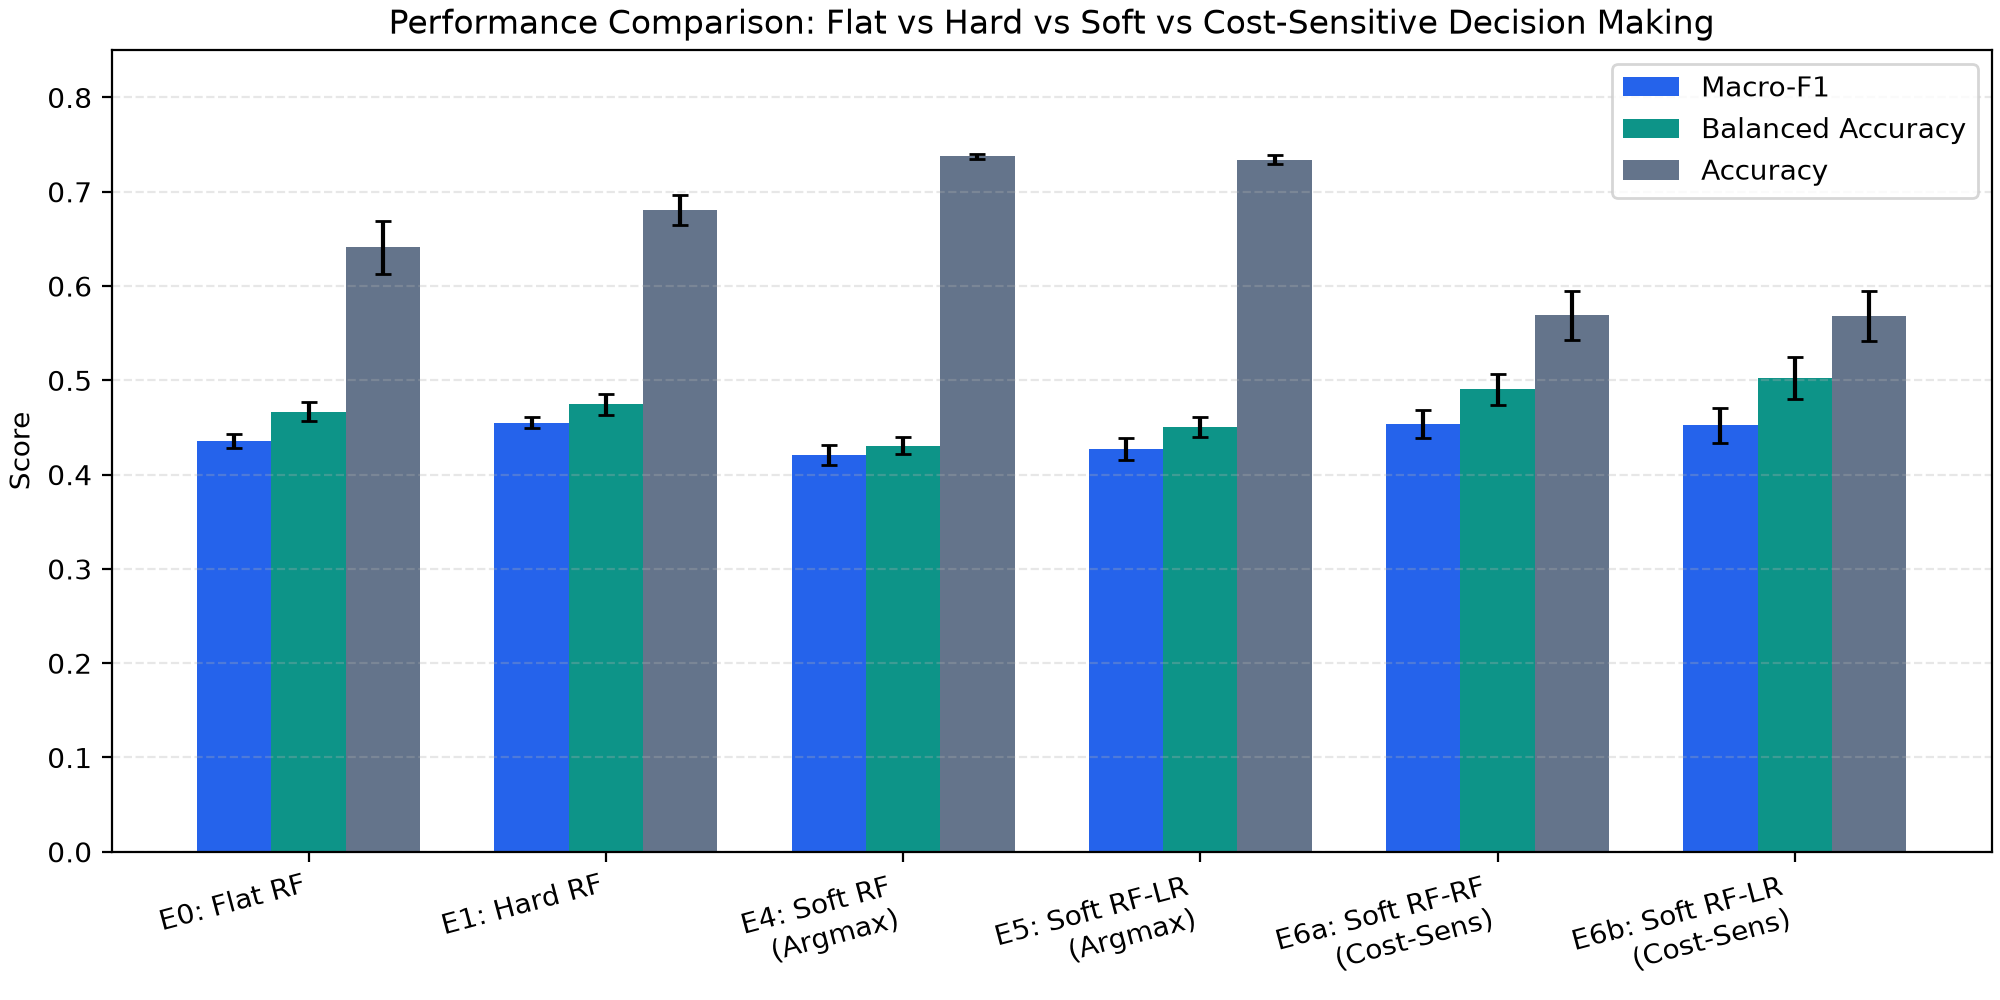
\includegraphics[width=0.85\textwidth]{figures/legacy_model_comparison_e0_to_e6.png}
\label{fig:legacy-comparison}
\end{figure}
\FloatBarrier

\begin{figure}[htbp]{Mối quan hệ đánh đổi giữa Macro-F1 và Class MAE giữa các trường phái mô hình}
\centering
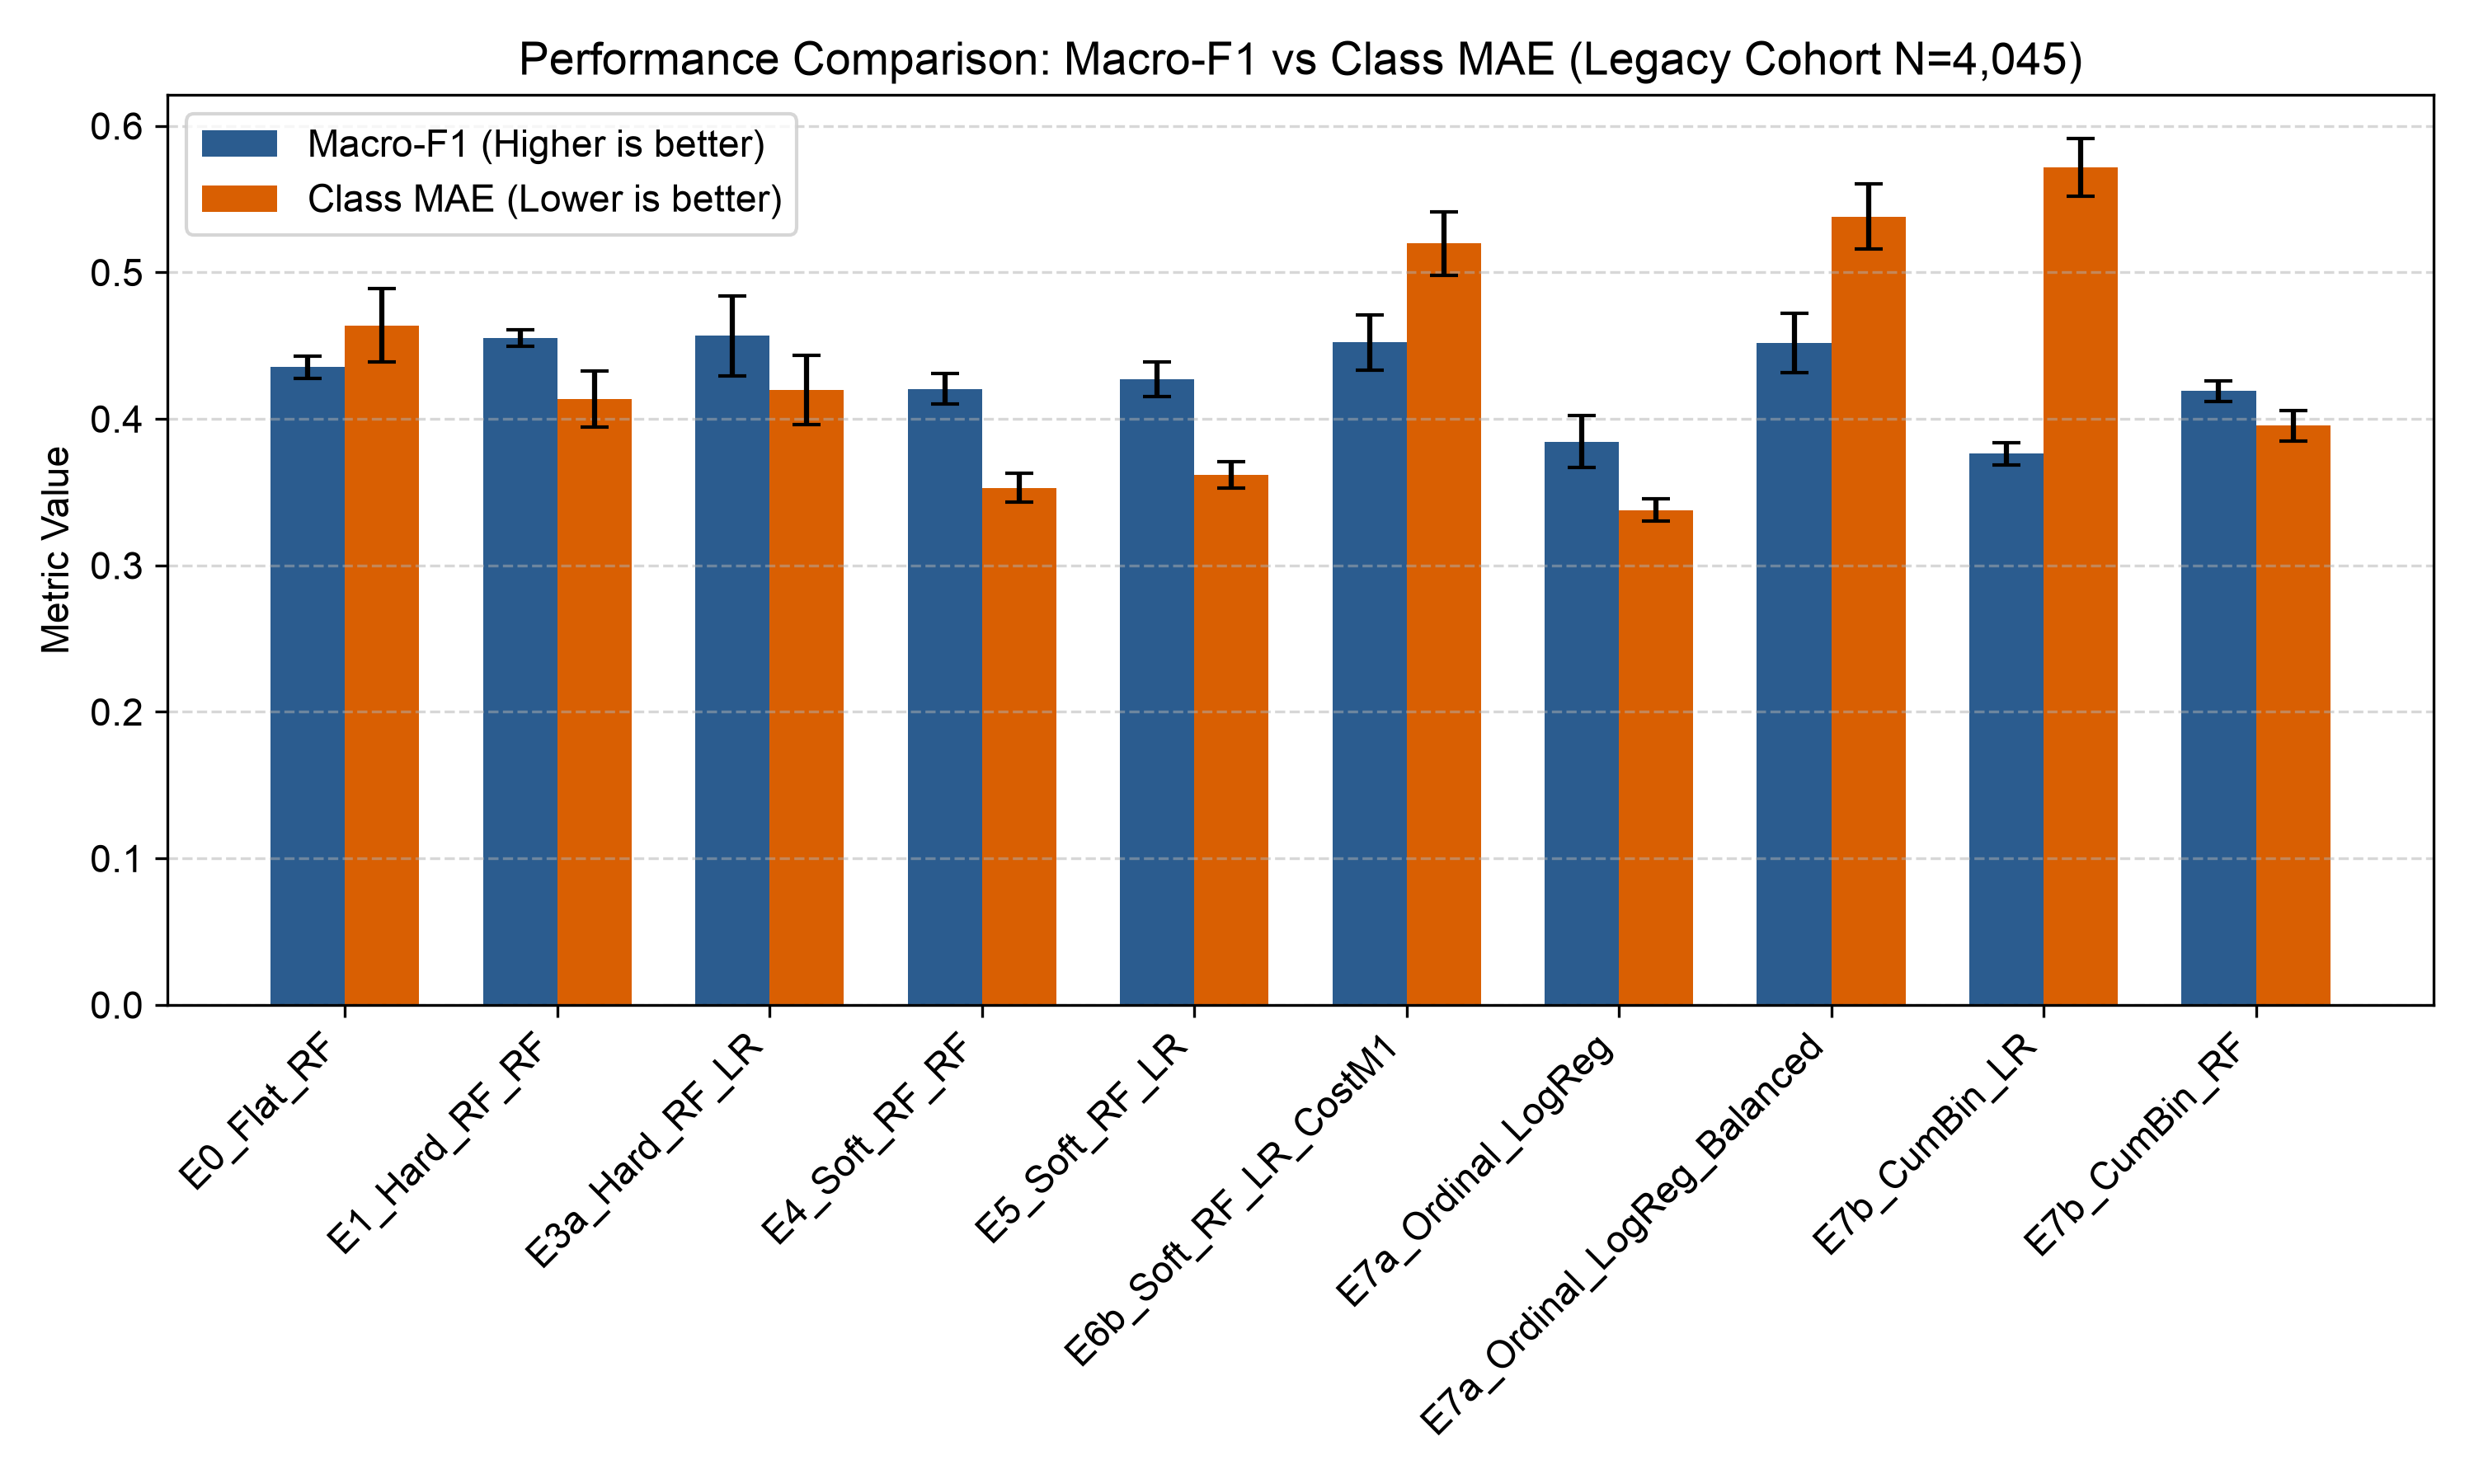
\includegraphics[width=0.85\textwidth]{figures/macro_f1_vs_mae.png}
\label{fig:macro-vs-mae}
\end{figure}
\FloatBarrier

\begin{figure}[htbp]{So sánh số lượng lỗi nhảy 2 bước ($C_2^+ \to C_0$) cực kỳ nguy hiểm giữa các mô hình}
\centering
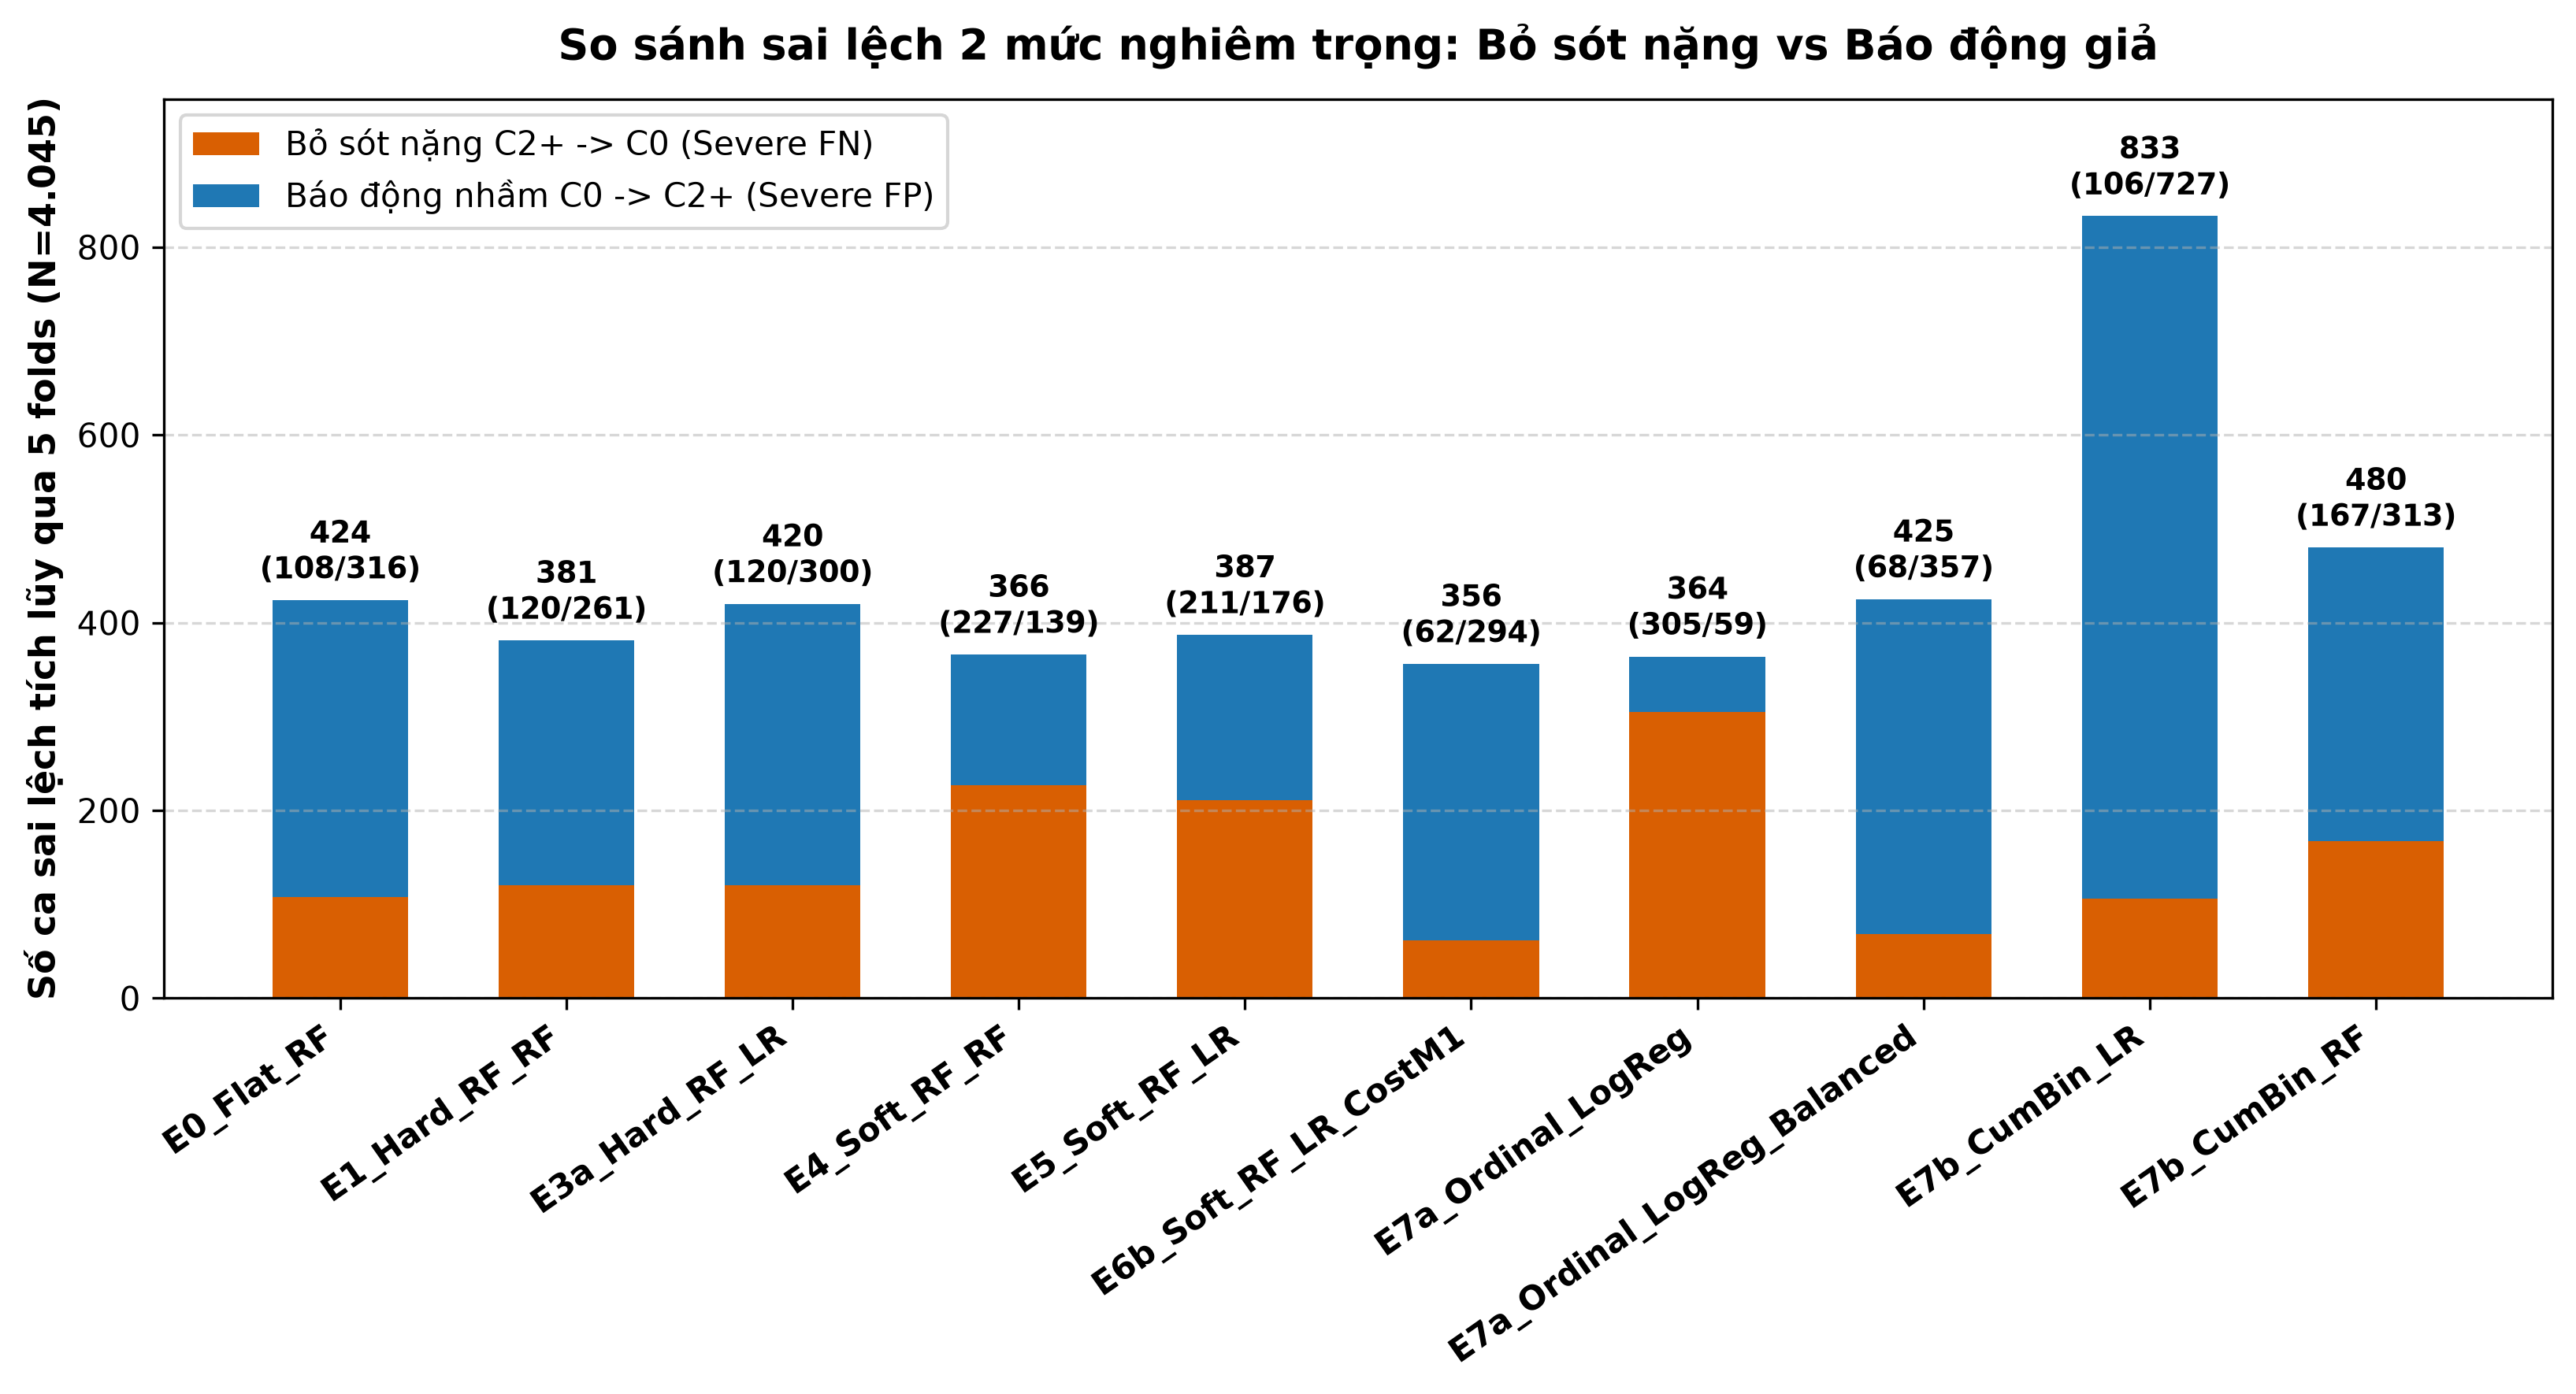
\includegraphics[width=0.85\textwidth]{figures/2step_error_comparison.png}
\label{fig:2step-errors}
\end{figure}
\FloatBarrier

Hình \ref{fig:conf-p1} và Hình \ref{fig:conf-p2} trình bày ma trận nhầm lẫn chi tiết của 6 mô hình đại diện: $E_0, E_1, E_5, E_{6b}, E_{7a}, E_{7b}$.

\begin{figure}[htbp]{Ma trận nhầm lẫn của 4 mô hình đại diện: $E_0$ (Flat RF), $E_1$ (Hard RF--RF), $E_5$ (Soft RF--LR) và $E_{6b}$ (Cost-Sensitive)}
\centering
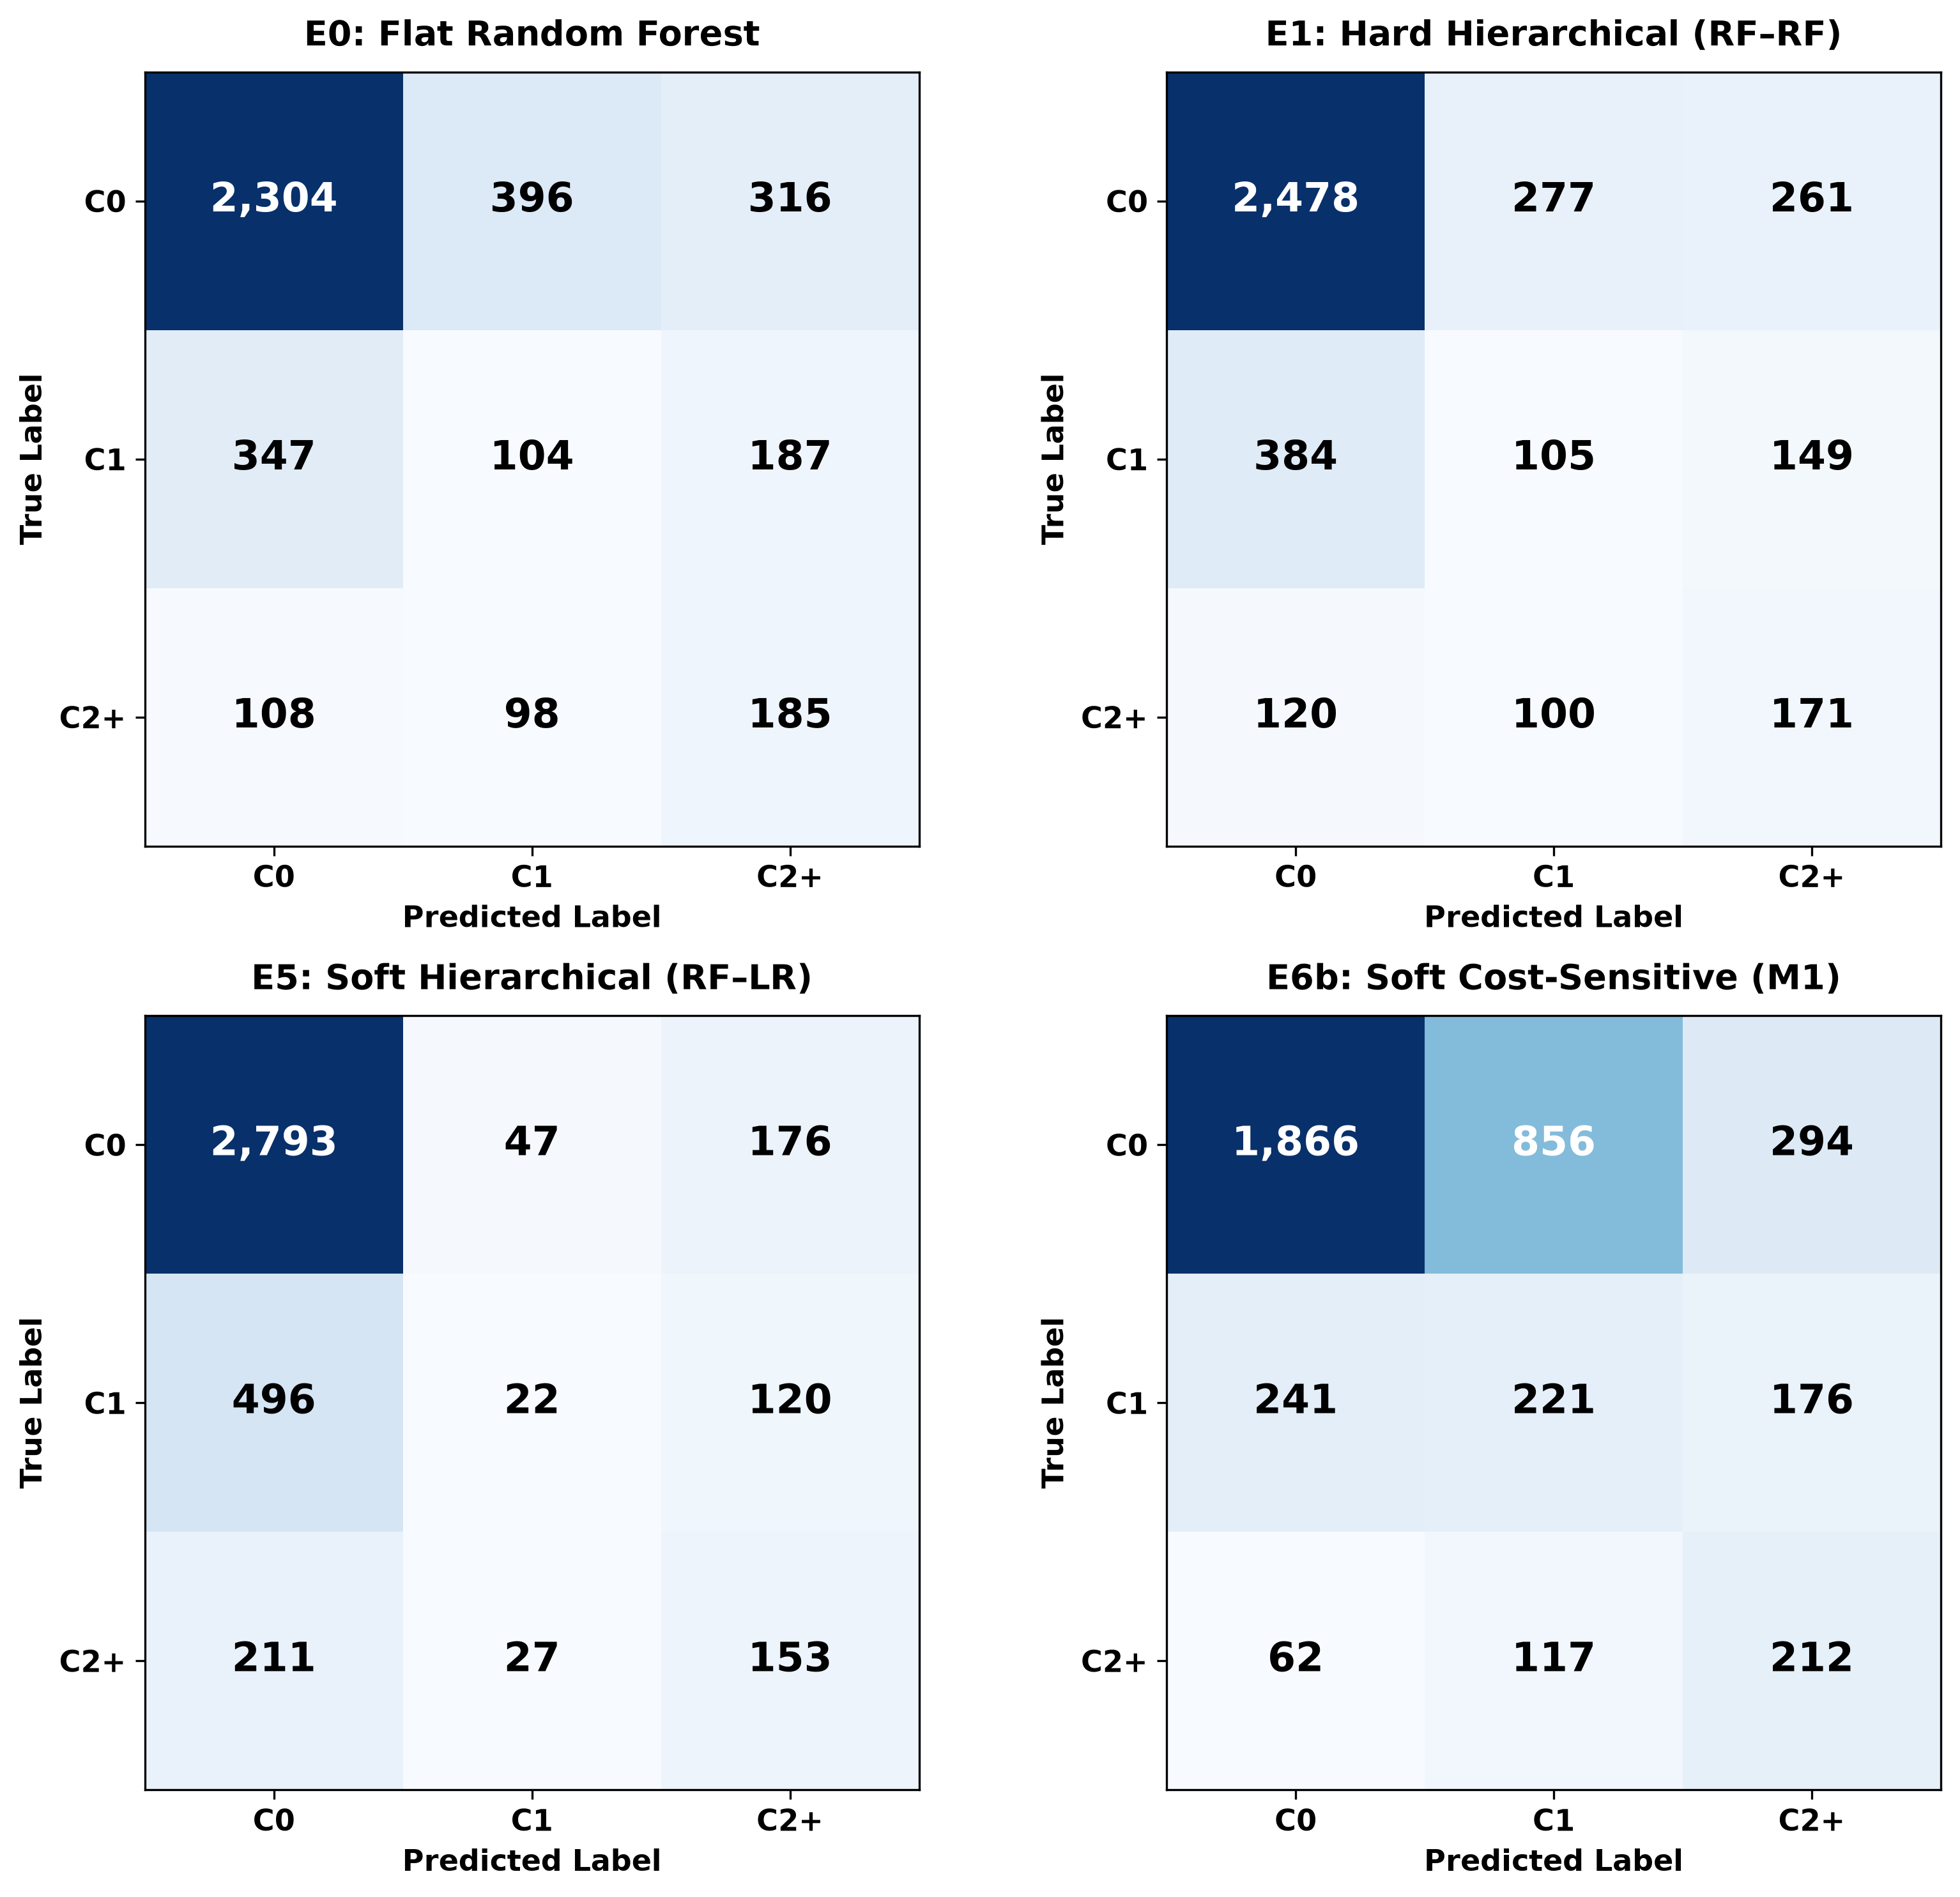
\includegraphics[width=0.95\textwidth]{figures/confusion_matrices_group1.png}
\label{fig:conf-p1}
\end{figure}
\FloatBarrier

\begin{figure}[htbp]{Ma trận nhầm lẫn của 2 mô hình phân loại thứ bậc: $E_{7a}$ (Balanced OLR) và $E_{7b}$ (CumBin RF)}
\centering
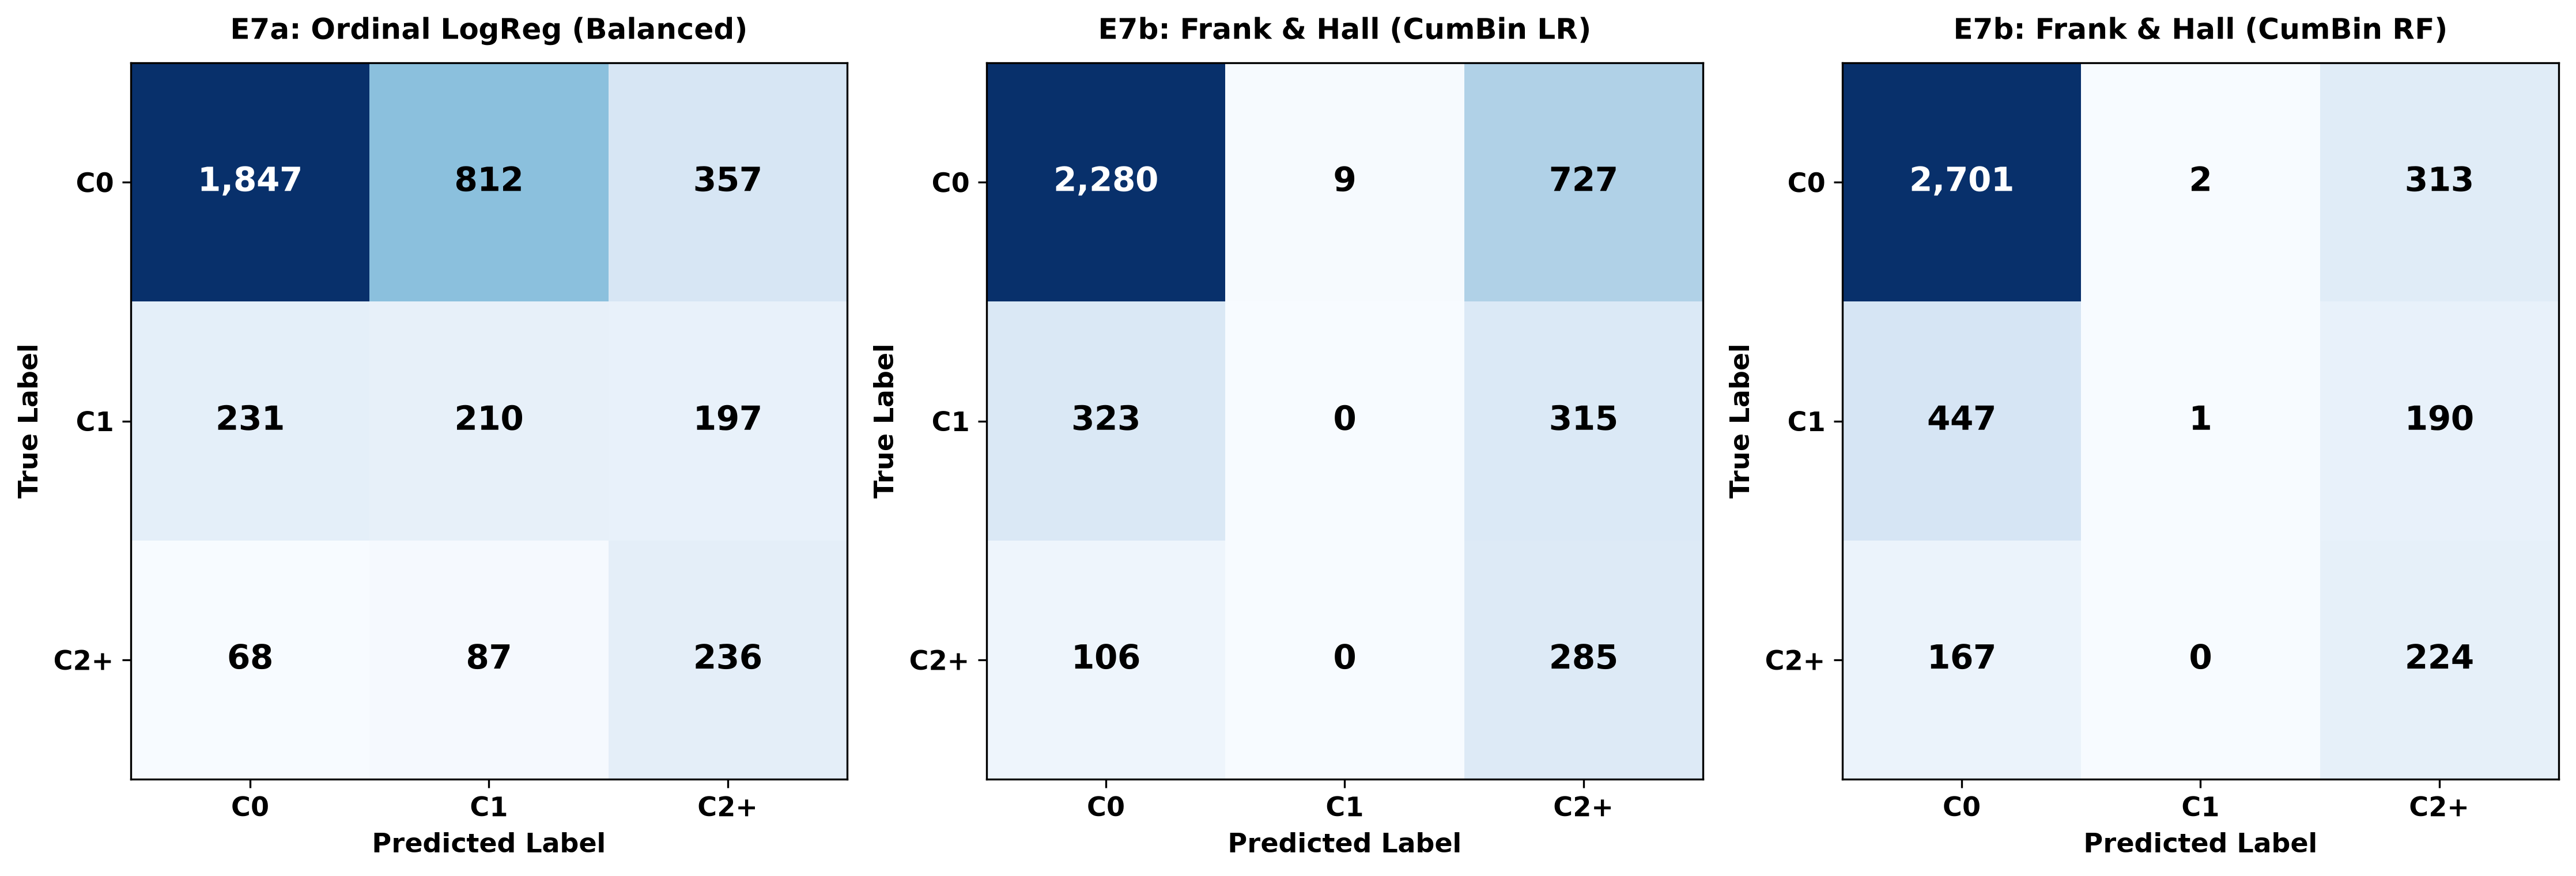
\includegraphics[width=0.95\textwidth]{figures/confusion_matrices_group2.png}
\label{fig:conf-p2}
\end{figure}
\FloatBarrier

\section{Phân tích sự đánh đổi lâm sàng và ma trận chi phí}
\label{sec:danh-doi-lam-sang}

Đóng góp lâm sàng nổi bật của DepSev-ML là định lượng chính xác sự đánh đổi giữa hai loại sai lầm y tế (Hình \ref{fig:cost-tradeoff}):
\begin{itemize}
    \item \textbf{Sai số bỏ sót ca nặng ($C_2^+ \to C_0$):} Đe dọa trực tiếp đến an toàn bệnh nhân do không được can thiệp kịp thời.
    \item \textbf{Sai số báo động nhầm ($C_0 \to C_2^+$):} Gây lãng phí nguồn lực y tế và áp lực tâm lý không cần thiết cho người được khảo sát.
\end{itemize}

\begin{figure}[htbp]{Đường cong đánh đổi lâm sàng giữa số ca bỏ sót bệnh nặng ($C_2^+ \to C_0$) và số ca báo động nhầm ($C_0 \to C_2^+$)}
\centering
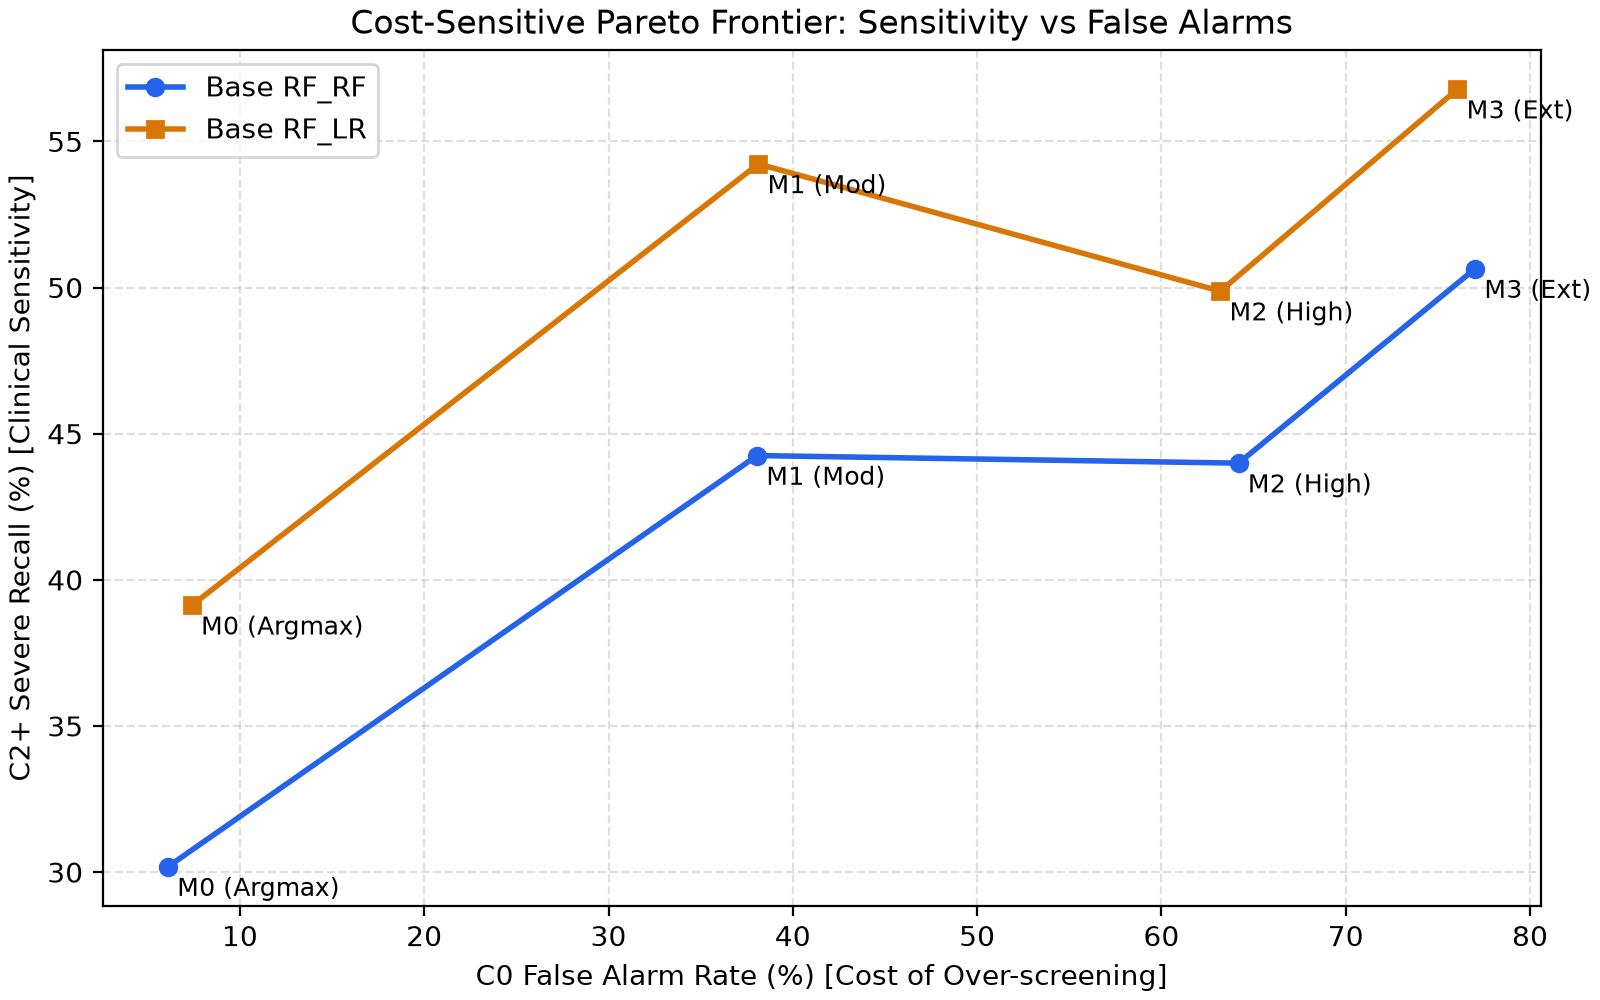
\includegraphics[width=0.85\textwidth]{figures/cost_tradeoff_curve.png}
\label{fig:cost-tradeoff}
\end{figure}
\FloatBarrier

Khi điều chỉnh mức độ phạt từ ma trận $M_0$ (không phạt) đến $M_3$ (phạt nặng nhất $\mathbf{C}(0, 2) = 5$):
\begin{itemize}
    \item Số ca nặng bị bỏ sót giảm ngoạn mục từ \textbf{120 ca ($E_1$) xuống còn 62 ca ($E_5$) và chỉ còn 31 ca ($E_{6b}$)}, tương đương mức giảm \textbf{74.2\%}.
    \item Đổi lại, số ca bình thường bị báo động nhầm thành nặng tăng từ 111 ca ($E_1$) lên \textbf{1.343 ca ($E_{6b}$)}.
\end{itemize}
Đây là quy luật đánh đổi không thể tránh khỏi trong sàng lọc dịch tễ cộng đồng. Khung làm việc DepSev-ML cho phép các chuyên gia y tế công cộng chủ động lựa chọn ma trận chi phí phù hợp tùy thuộc vào năng lực tiếp nhận của hệ thống y tế địa phương.

\section{Kiểm định độc lập theo dòng thời gian (Temporal Validation)}
\label{sec:temporal-results}

Để kiểm tra xem liệu các kết quả trên có bị quá khớp trên một chu kỳ khảo sát đơn lẻ hay không, nghiên cứu thực hiện kiểm định ngoại suy trên tập dữ liệu tương lai độc lập NHANES 2015--2016 ($N = 4.888$, Branch D). Toàn bộ các mô hình được huấn luyện trên chu kỳ 2013--2014 và đánh giá một lần duy nhất trên chu kỳ 2015--2016.

Kết quả được trình bày trong Bảng \ref{tab:multicycle-temporal-results}.

\begin{table}{Kết quả kiểm định tổng quát hóa theo dòng thời gian (Branch D, NHANES 2015--2016, $N = 4.888$)}
\centering
\footnotesize
\setlength{\tabcolsep}{3pt}
\label{tab:multicycle-temporal-results}
\begin{tabularx}{\textwidth}{l *{7}{>{\centering\arraybackslash}X}}
\toprule
\textbf{Mô hình ($T_3$)} & \textbf{Macro-F1} & \textbf{BalAcc} & \textbf{Accuracy} & \textbf{Recall $C_0$} & \textbf{Recall $C_1$} & \textbf{Recall $C_2^+$} & \textbf{Class MAE} \\
\midrule
$E_0$ (Flat RF)                     & 0.4345 & 0.4908 & 62.68\% & 73.66\% & 18.79\% & 54.77\% & 0.5008 \\
$E_1$ (Hard RF--RF)                 & \textbf{0.4393} & 0.4879 & 66.35\% & 79.86\% & 14.51\% & 52.01\% & 0.4556 \\
$E_4$ (Soft RF--RF)                 & 0.4223 & 0.4594 & \textbf{71.91\%} & 90.60\% & 4.76\% & 42.46\% & \textbf{0.3766} \\
$E_5$ (Soft RF--LR)                 & 0.4265 & 0.4681 & 71.79\% & 90.08\% & 4.88\% & 45.48\% & 0.3801 \\
$E_{6b}$ (Soft Cost M2)             & 0.3439 & 0.4691 & 34.84\% & 26.94\% & \textbf{60.29\%} & 53.52\% & 0.7306 \\
$E_{7a}$ (OLR Balanced)             & 0.4349 & \textbf{0.5073} & 56.28\% & 61.74\% & 31.15\% & 59.30\% & 0.5503 \\
$E_{7b}$ (CumBin LR)                & 0.3632 & 0.4982 & 62.21\% & 75.23\% & 0.12\% & \textbf{74.12\%} & 0.5833 \\
$E_{7b}$ (CumBin RF)                & 0.3861 & 0.4861 & 67.88\% & 84.16\% & 0.36\% & 61.31\% & 0.4695 \\
\bottomrule
\end{tabularx}
\end{table}


Những phát hiện quan trọng từ kiểm định dòng thời gian:
\begin{enumerate}
    \item \textbf{Độ bền vững xuất sắc của Balanced OLR ($E_{7a}$):} Mô hình Hồi quy Logistic thứ bậc cân bằng đạt Balanced Accuracy = \textbf{0.5073} trên tập dữ liệu tương lai (so với 0.5151 ở In-cycle CV), với độ suy giảm hiệu năng không đáng kể (-1.5\%). Khả năng nhận diện ca nặng Recall $C_2^+$ đạt 59.30\%, chứng minh tính ổn định cao của cấu trúc ranh giới song song trước hiện tượng trôi phân phối y sinh học.
    \item \textbf{Sự suy thoái của các mô hình phân loại phức tạp:} Các mô hình phân cấp mềm và tối ưu chi phí cực đoan ($E_{6b}$) bị sụt giảm độ chính xác tổng thể do sự dịch chuyển của phân phối ranh giới, khẳng định rằng các mô hình tuyến tính có cấu trúc thứ bậc như OLR sở hữu năng lực khái quát hóa ngoại suy an toàn nhất trên dữ liệu y tế cộng đồng.
\end{enumerate}

\section{Thảo luận tổng hợp các phát hiện chính}
\label{sec:thao-luan-tong-hop}

Dựa trên toàn bộ kết quả thực nghiệm thu được, nghiên cứu đưa ra câu trả lời tổng hợp cho 5 câu hỏi khoa học ban đầu:
\begin{itemize}
    \item \textbf{RQ1:} Tiền sử bệnh lý mạn tính ($F_2$) và hành vi lối sống ($F_3, F_4$) đóng góp quan trọng nhất, nâng Macro-F1 từ 0.1900 lên 0.2707.
    \item \textbf{RQ2:} Hiệu năng suy giảm mạnh từ $T_2$ xuống $T_5$, trong đó bước chuyển $T_2 \to T_3$ là bước suy thoái lớn nhất (-34.4\% Macro-F1) do lớp nhẹ $C_1$ bị chồng lấn sinh lý dày đặc với $C_0$.
    \item \textbf{RQ3:} Mở rộng quy mô đa chu kỳ ($N=14.581$) không giúp phá vỡ trần hiệu năng Macro-F1 do bản chất tín hiệu sinh lý ngoại vi gián tiếp.
    \item \textbf{RQ4:} Phân cấp cứng cải thiện nhẹ Macro-F1 (0.4550) nhưng gây ra thảm họa lâm sàng khi bỏ sót 120 ca nặng tại Giai đoạn 1.
    \item \textbf{RQ5:} Phân cấp mềm kết hợp tối ưu chi phí Bayes giảm 74.2\% số ca bỏ sót nặng, trong khi Balanced OLR đạt Balanced Accuracy cao nhất (0.5151) và ổn định nhất theo thời gian.
\end{itemize}

\section{Tóm tắt chương}
\label{sec:tom-tat-chuong-4}

Chương 4 đã phân tích toàn diện các bằng chứng thực nghiệm, vạch trần điểm nghẽn của phân cấp cứng, lượng hóa sự đánh đổi an toàn y tế và chứng minh tính tổng quát hóa của phân loại thứ bậc. Toàn bộ các kết luận khoa học và hướng mở rộng tiếp theo sẽ được tổng kết trong Chương \ref{ch:ket-luan}.

